\documentclass{book}
\usepackage[a4paper,top=2.5cm,bottom=2.5cm,left=2.5cm,right=2.5cm]{geometry}
\usepackage{makeidx}
\usepackage{natbib}
\usepackage{graphicx}
\usepackage{multicol}
\usepackage{float}
\usepackage{listings}
\usepackage{color}
\usepackage{ifthen}
\usepackage[table]{xcolor}
\usepackage{textcomp}
\usepackage{alltt}
\usepackage{ifpdf}
\ifpdf
\usepackage[pdftex,
            pagebackref=true,
            colorlinks=true,
            linkcolor=blue,
            unicode
           ]{hyperref}
\else
\usepackage[ps2pdf,
            pagebackref=true,
            colorlinks=true,
            linkcolor=blue,
            unicode
           ]{hyperref}
\usepackage{pspicture}
\fi
\usepackage[utf8]{inputenc}
\usepackage{mathptmx}
\usepackage[scaled=.90]{helvet}
\usepackage{courier}
\usepackage{sectsty}
\usepackage{amssymb}
\usepackage[titles]{tocloft}
\usepackage{doxygen}
\lstset{language=C++,inputencoding=utf8,basicstyle=\footnotesize,breaklines=true,breakatwhitespace=true,tabsize=4,numbers=left }
\makeindex
\setcounter{tocdepth}{3}
\renewcommand{\footrulewidth}{0.4pt}
\renewcommand{\familydefault}{\sfdefault}
\hfuzz=15pt
\setlength{\emergencystretch}{15pt}
\hbadness=750
\tolerance=750
\begin{document}
\hypersetup{pageanchor=false,citecolor=blue}
\begin{titlepage}
\vspace*{7cm}
\begin{center}
{\Large Deferred Shading Renderer \\[1ex]\large v.\-03 }\\
\vspace*{1cm}
{\large Generated by Doxygen 1.8.2}\\
\vspace*{0.5cm}
{\small Thu Dec 13 2012 15:57:45}\\
\end{center}
\end{titlepage}
\clearemptydoublepage
\pagenumbering{roman}
\tableofcontents
\clearemptydoublepage
\pagenumbering{arabic}
\hypersetup{pageanchor=true,citecolor=blue}
\chapter{Todo List}
\label{todo}
\hypertarget{todo}{}

\begin{DoxyRefList}
\item[\label{todo__todo000001}%
\hypertarget{todo__todo000001}{}%
File \hyperlink{_cone_light_volume_8h}{Cone\-Light\-Volume.h} ]Implement method to return the factor needed in light direction calculation 

Finish the algorithm for Y,Z rotations 

Add a method using Mat4 $\ast$ Vec4 for cone positioning based on a pre-\/given aim vector.  
\item[\label{todo__todo000002}%
\hypertarget{todo__todo000002}{}%
File \hyperlink{_deferred_shading_8h}{Deferred\-Shading.h} ]Change the O\-B\-J\-Loader array with a vector since we can have 

for example 20 pointlights each with its shader.  
\item[\label{todo__todo000003}%
\hypertarget{todo__todo000003}{}%
Class \hyperlink{classngl_1_1_light}{ngl\-:\-:Light} ]this will need to be changed to work with G\-L\-S\-L lights for G\-L\-\_\-\-V\-E\-R\-S\-I\-O\-N $>$ 3.\-x  
\item[\label{todo__todo000004}%
\hypertarget{todo__todo000004}{}%
File \hyperlink{_object_loader_8h}{Object\-Loader.h} ]
\item[\label{todo__todo000005}%
\hypertarget{todo__todo000005}{}%
File \hyperlink{_sphere_light_volume_8h}{Sphere\-Light\-Volume.h} ]
\item[\label{todo__todo000006}%
\hypertarget{todo__todo000006}{}%
File \hyperlink{_spot_light_8h}{Spot\-Light.h} ]
\end{DoxyRefList}
\chapter{Hierarchical Index}
\section{Class Hierarchy}
This inheritance list is sorted roughly, but not completely, alphabetically\-:\begin{DoxyCompactList}
\item \contentsline{section}{Cone\-Light\-Volume}{\pageref{class_cone_light_volume}}{}
\item \contentsline{section}{Deferred\-Shading}{\pageref{class_deferred_shading}}{}
\item \contentsline{section}{ngl\-:\-:Light}{\pageref{classngl_1_1_light}}{}
\item \contentsline{section}{Object\-Loader}{\pageref{class_object_loader}}{}
\item Q\-G\-L\-Widget\begin{DoxyCompactList}
\item \contentsline{section}{G\-L\-Window}{\pageref{class_g_l_window}}{}
\end{DoxyCompactList}
\item Q\-Main\-Window\begin{DoxyCompactList}
\item \contentsline{section}{Main\-Window}{\pageref{class_main_window}}{}
\end{DoxyCompactList}
\item \contentsline{section}{Sphere\-Light\-Volume}{\pageref{class_sphere_light_volume}}{}
\item \contentsline{section}{Spotlight}{\pageref{class_spotlight}}{}
\end{DoxyCompactList}

\chapter{Class Index}
\section{Class List}
Here are the classes, structs, unions and interfaces with brief descriptions\-:\begin{DoxyCompactList}
\item\contentsline{section}{\hyperlink{class_cone_light_volume}{Cone\-Light\-Volume} }{\pageref{class_cone_light_volume}}{}
\item\contentsline{section}{\hyperlink{class_deferred_shading}{Deferred\-Shading} }{\pageref{class_deferred_shading}}{}
\item\contentsline{section}{\hyperlink{class_g_l_window}{G\-L\-Window} \\*Our main glwindow widget for N\-G\-L applications all drawing elements are put in this file }{\pageref{class_g_l_window}}{}
\item\contentsline{section}{\hyperlink{classngl_1_1_light}{ngl\-::\-Light} \\*Simple class to encapsulate Open\-G\-L \hyperlink{classngl_1_1_light}{Light} functions this will fill in the following structure }{\pageref{classngl_1_1_light}}{}
\item\contentsline{section}{\hyperlink{class_main_window}{Main\-Window} \\*Main re-\/sizable window which contains a \hyperlink{class_g_l_window}{G\-L\-Window} widget used to hold our basic gl applications }{\pageref{class_main_window}}{}
\item\contentsline{section}{\hyperlink{class_object_loader}{Object\-Loader} }{\pageref{class_object_loader}}{}
\item\contentsline{section}{\hyperlink{class_sphere_light_volume}{Sphere\-Light\-Volume} }{\pageref{class_sphere_light_volume}}{}
\item\contentsline{section}{\hyperlink{class_spotlight}{Spotlight} }{\pageref{class_spotlight}}{}
\end{DoxyCompactList}

\chapter{File Index}
\section{File List}
Here is a list of all documented files with brief descriptions\-:\begin{DoxyCompactList}
\item\contentsline{section}{C\-:/\-N\-G\-L/\-Projects/\-Deferred\-Renderer/include/\hyperlink{_cone_light_volume_8h}{Cone\-Light\-Volume.\-h} }{\pageref{_cone_light_volume_8h}}{}
\item\contentsline{section}{C\-:/\-N\-G\-L/\-Projects/\-Deferred\-Renderer/include/\hyperlink{_deferred_shading_8h}{Deferred\-Shading.\-h} }{\pageref{_deferred_shading_8h}}{}
\item\contentsline{section}{C\-:/\-N\-G\-L/\-Projects/\-Deferred\-Renderer/include/\hyperlink{_g_l_window_8h}{G\-L\-Window.\-h} \\*Basic Qt G\-L window class for ngl demos }{\pageref{_g_l_window_8h}}{}
\item\contentsline{section}{C\-:/\-N\-G\-L/\-Projects/\-Deferred\-Renderer/include/\hyperlink{_main_window_8h}{Main\-Window.\-h} \\*This is the \hyperlink{class_main_window}{Main\-Window} Class which is generated by the Ui file, if we wish to add anything to the main Ui we add it here }{\pageref{_main_window_8h}}{}
\item\contentsline{section}{C\-:/\-N\-G\-L/\-Projects/\-Deferred\-Renderer/include/\hyperlink{_object_loader_8h}{Object\-Loader.\-h} }{\pageref{_object_loader_8h}}{}
\item\contentsline{section}{C\-:/\-N\-G\-L/\-Projects/\-Deferred\-Renderer/include/\hyperlink{_sphere_light_volume_8h}{Sphere\-Light\-Volume.\-h} }{\pageref{_sphere_light_volume_8h}}{}
\item\contentsline{section}{C\-:/\-N\-G\-L/\-Projects/\-Deferred\-Renderer/include/\hyperlink{_spot_light_8h}{Spot\-Light.\-h} }{\pageref{_spot_light_8h}}{}
\item\contentsline{section}{C\-:/\-N\-G\-L/\-Projects/\-Deferred\-Renderer/include/ngl/\hyperlink{_light_8h}{Light.\-h} \\*Encapsulation of an Open\-G\-L Light }{\pageref{_light_8h}}{}
\end{DoxyCompactList}

\chapter{Class Documentation}
\hypertarget{class_cone_light_volume}{\section{Cone\-Light\-Volume Class Reference}
\label{class_cone_light_volume}\index{Cone\-Light\-Volume@{Cone\-Light\-Volume}}
}
\subsection*{Public Member Functions}
\begin{DoxyCompactItemize}
\item 
\hyperlink{class_cone_light_volume_ab8626d8dc7a7acaf9c5c499f5ee10c07}{Cone\-Light\-Volume} (ngl\-::\-Vec3 \-\_\-light\-Position, ngl\-::\-Colour \-\_\-light\-Intensity, ngl\-::\-Real \-\_\-cone\-Radius, ngl\-::\-Real \-\_\-cone\-Height, ngl\-::\-Vec3 \-\_\-cone\-Orientation)
\begin{DoxyCompactList}\small\item\em ctor for creating a Cone volume for the light. \end{DoxyCompactList}\item 
\hypertarget{class_cone_light_volume_ac3227dccbeb84973aba06381f5b3f750}{\hyperlink{class_cone_light_volume_ac3227dccbeb84973aba06381f5b3f750}{$\sim$\-Cone\-Light\-Volume} ()}\label{class_cone_light_volume_ac3227dccbeb84973aba06381f5b3f750}

\begin{DoxyCompactList}\small\item\em default dtor \end{DoxyCompactList}\item 
\hypertarget{class_cone_light_volume_a34d75c868c3797bb8d218ec4e4424231}{ngl\-::\-Vec2 \hyperlink{class_cone_light_volume_a34d75c868c3797bb8d218ec4e4424231}{get\-Radius\-And\-Heigth} () const }\label{class_cone_light_volume_a34d75c868c3797bb8d218ec4e4424231}

\begin{DoxyCompactList}\small\item\em Returns the Radius and Height. \end{DoxyCompactList}\item 
\hypertarget{class_cone_light_volume_a25eb3fece7c140c43c4672045773f408}{ngl\-::\-Vec3 \hyperlink{class_cone_light_volume_a25eb3fece7c140c43c4672045773f408}{get\-New\-Position} () const }\label{class_cone_light_volume_a25eb3fece7c140c43c4672045773f408}

\begin{DoxyCompactList}\small\item\em Returns the New Position Coordinates. \end{DoxyCompactList}\item 
\hypertarget{class_cone_light_volume_ab90a22c87d468647a6cce9a555c5b4be}{ngl\-::\-Vec3 \hyperlink{class_cone_light_volume_ab90a22c87d468647a6cce9a555c5b4be}{get\-Cone\-Orientation} () const }\label{class_cone_light_volume_ab90a22c87d468647a6cce9a555c5b4be}

\begin{DoxyCompactList}\small\item\em Returns the New Cone Orientation. \end{DoxyCompactList}\end{DoxyCompactItemize}


\subsection{Constructor \& Destructor Documentation}
\hypertarget{class_cone_light_volume_ab8626d8dc7a7acaf9c5c499f5ee10c07}{\index{Cone\-Light\-Volume@{Cone\-Light\-Volume}!Cone\-Light\-Volume@{Cone\-Light\-Volume}}
\index{Cone\-Light\-Volume@{Cone\-Light\-Volume}!ConeLightVolume@{Cone\-Light\-Volume}}
\subsubsection[{Cone\-Light\-Volume}]{\setlength{\rightskip}{0pt plus 5cm}Cone\-Light\-Volume\-::\-Cone\-Light\-Volume (
\begin{DoxyParamCaption}
\item[{ngl\-::\-Vec3}]{\-\_\-light\-Position, }
\item[{ngl\-::\-Colour}]{\-\_\-light\-Intensity, }
\item[{ngl\-::\-Real}]{\-\_\-cone\-Radius, }
\item[{ngl\-::\-Real}]{\-\_\-cone\-Height, }
\item[{ngl\-::\-Vec3}]{\-\_\-cone\-Orientation}
\end{DoxyParamCaption}
)}}\label{class_cone_light_volume_ab8626d8dc7a7acaf9c5c499f5ee10c07}


ctor for creating a Cone volume for the light. 

Reguired parameters\-: light position light intensity cone radius cone height cone orientation in degrees 

The documentation for this class was generated from the following files\-:\begin{DoxyCompactItemize}
\item 
C\-:/\-N\-G\-L/\-Projects/\-Deferred\-Renderer/include/\hyperlink{_cone_light_volume_8h}{Cone\-Light\-Volume.\-h}\item 
C\-:/\-N\-G\-L/\-Projects/\-Deferred\-Renderer/src/Cone\-Light\-Volume.\-cpp\end{DoxyCompactItemize}

\hypertarget{class_deferred_shading}{\section{Deferred\-Shading Class Reference}
\label{class_deferred_shading}\index{Deferred\-Shading@{Deferred\-Shading}}
}
\subsection*{Public Member Functions}
\begin{DoxyCompactItemize}
\item 
\hypertarget{class_deferred_shading_ab7d27bb57a296dcd0927b8382bd75d5f}{\hyperlink{class_deferred_shading_ab7d27bb57a296dcd0927b8382bd75d5f}{Deferred\-Shading} (int \-\_\-width, int \-\_\-height)}\label{class_deferred_shading_ab7d27bb57a296dcd0927b8382bd75d5f}

\begin{DoxyCompactList}\small\item\em ctor setting the same window size as the main application \end{DoxyCompactList}\item 
\hypertarget{class_deferred_shading_ac237f4f2a96e2d9871011f9c9978af85}{\hyperlink{class_deferred_shading_ac237f4f2a96e2d9871011f9c9978af85}{$\sim$\-Deferred\-Shading} ()}\label{class_deferred_shading_ac237f4f2a96e2d9871011f9c9978af85}

\begin{DoxyCompactList}\small\item\em dtor removing all the pointer that are created \end{DoxyCompactList}\item 
\hypertarget{class_deferred_shading_a2fad3267f5e62743175e6f430257ca3a}{void \hyperlink{class_deferred_shading_a2fad3267f5e62743175e6f430257ca3a}{init\-Scene} ()}\label{class_deferred_shading_a2fad3267f5e62743175e6f430257ca3a}

\begin{DoxyCompactList}\small\item\em Initializng Scene. \end{DoxyCompactList}\item 
\hypertarget{class_deferred_shading_ab64677da33f7c88f08520b38497eabfa}{void \hyperlink{class_deferred_shading_ab64677da33f7c88f08520b38497eabfa}{set\-Resize\-Scene} (int \&\-\_\-width, int \&\-\_\-height)}\label{class_deferred_shading_ab64677da33f7c88f08520b38497eabfa}

\begin{DoxyCompactList}\small\item\em Set width and height for re-\/draw. \end{DoxyCompactList}\item 
void \hyperlink{class_deferred_shading_ae61c4970e594173bfe657b8e072cf056}{load\-Deferred\-Shader} (G\-Lint \-\_\-shader\-Number, std\-::string \-\_\-shader\-Program\-Name, std\-::string \-\_\-vertex\-Shader\-File\-Name, std\-::string \-\_\-fragment\-Shader\-File\-Name)
\begin{DoxyCompactList}\small\item\em Load the specified shaders for light computation. \end{DoxyCompactList}\item 
\hypertarget{class_deferred_shading_a6da63e5d421410d9f6a340bba0f9f051}{void \hyperlink{class_deferred_shading_a6da63e5d421410d9f6a340bba0f9f051}{set\-Camera\-Location} (ngl\-::\-Camera $\ast$\-\_\-camera)}\label{class_deferred_shading_a6da63e5d421410d9f6a340bba0f9f051}

\begin{DoxyCompactList}\small\item\em Save our camera location to be used when calculating the different lights. \end{DoxyCompactList}\item 
\hypertarget{class_deferred_shading_a4c11b2929a2b9497ef3e69645e4c887e}{void \hyperlink{class_deferred_shading_a4c11b2929a2b9497ef3e69645e4c887e}{start\-Deferred\-Frame} ()}\label{class_deferred_shading_a4c11b2929a2b9497ef3e69645e4c887e}

\begin{DoxyCompactList}\small\item\em Setup the renderer to process a new frame. \end{DoxyCompactList}\item 
\hypertarget{class_deferred_shading_a9cc19ee2fb7f38e86481b75963cf74cc}{void \hyperlink{class_deferred_shading_a9cc19ee2fb7f38e86481b75963cf74cc}{do\-Geometry\-Pass} ()}\label{class_deferred_shading_a9cc19ee2fb7f38e86481b75963cf74cc}

\begin{DoxyCompactList}\small\item\em Setup the renderer for Geometry pass. \end{DoxyCompactList}\item 
\hypertarget{class_deferred_shading_a4424578aceef5203ad155fc405fd24ef}{void \hyperlink{class_deferred_shading_a4424578aceef5203ad155fc405fd24ef}{start\-Stencil\-Point\-Light} (G\-Lint \&\-\_\-shader\-Number, ngl\-::\-Transform\-Stack \&\-\_\-tx, G\-Lint \&\-\_\-light\-Index)}\label{class_deferred_shading_a4424578aceef5203ad155fc405fd24ef}

\begin{DoxyCompactList}\small\item\em Setup the renderer for Point Lightning pass. \end{DoxyCompactList}\item 
\hypertarget{class_deferred_shading_ae9e5e37687b9a8658e99e97c86cc87fe}{void \hyperlink{class_deferred_shading_ae9e5e37687b9a8658e99e97c86cc87fe}{deferred\-Point\-Light} (G\-Lint \&\-\_\-shader\-Number, ngl\-::\-Transform\-Stack \&\-\_\-tx, G\-Lint \&\-\_\-light\-Index)}\label{class_deferred_shading_ae9e5e37687b9a8658e99e97c86cc87fe}

\begin{DoxyCompactList}\small\item\em Render the scene using the specified \-\_\-shader\-Number and the transformation stack using point light. \end{DoxyCompactList}\item 
\hypertarget{class_deferred_shading_aabd36b11f4659769486298e2c17d0d3a}{void \hyperlink{class_deferred_shading_aabd36b11f4659769486298e2c17d0d3a}{start\-Stencil\-Spot\-Light} (G\-Lint \&\-\_\-shader\-Number, ngl\-::\-Transform\-Stack \&\-\_\-tx, G\-Lint \&\-\_\-light\-Index)}\label{class_deferred_shading_aabd36b11f4659769486298e2c17d0d3a}

\begin{DoxyCompactList}\small\item\em Setup the renderer for Spot Lightning pass. \end{DoxyCompactList}\item 
\hypertarget{class_deferred_shading_a173c7b9f47fc7274f2959ec64f8baa56}{void \hyperlink{class_deferred_shading_a173c7b9f47fc7274f2959ec64f8baa56}{deferred\-Spot\-Light} (G\-Lint \&\-\_\-shader\-Number, ngl\-::\-Transform\-Stack \&\-\_\-tx, G\-Lint \&\-\_\-light\-Index)}\label{class_deferred_shading_a173c7b9f47fc7274f2959ec64f8baa56}

\begin{DoxyCompactList}\small\item\em Render the scene using the specified \-\_\-shader\-Number and the transformation stack using point light. \end{DoxyCompactList}\item 
\hypertarget{class_deferred_shading_a3e16121405f0218c7cfc0b48f7d96236}{void \hyperlink{class_deferred_shading_a3e16121405f0218c7cfc0b48f7d96236}{deferred\-Directional\-Light} (G\-Lint \&\-\_\-shader\-Number, G\-Lint \&\-\_\-light\-Index)}\label{class_deferred_shading_a3e16121405f0218c7cfc0b48f7d96236}

\begin{DoxyCompactList}\small\item\em Render the final scene using the specified \-\_\-shader\-Number and directional light. \end{DoxyCompactList}\item 
\hypertarget{class_deferred_shading_af8fb86b0971f5b2e0fbb01d0fdeb1351}{void \hyperlink{class_deferred_shading_af8fb86b0971f5b2e0fbb01d0fdeb1351}{deferred\-Light\-Final\-Pass} ()}\label{class_deferred_shading_af8fb86b0971f5b2e0fbb01d0fdeb1351}

\begin{DoxyCompactList}\small\item\em Render the final scene. \end{DoxyCompactList}\item 
\hypertarget{class_deferred_shading_a8032518b51fccbc065f2f545b219c799}{void \hyperlink{class_deferred_shading_a8032518b51fccbc065f2f545b219c799}{set\-Light\-In\-Scene} (G\-Lint \-\_\-shader\-Number, ngl\-::\-Vec3 \-\_\-light\-Position, ngl\-::\-Colour \-\_\-diffuse\-Color, ngl\-::\-Colour \-\_\-specular\-Color, ngl\-::\-L\-I\-G\-H\-T\-M\-O\-D\-E\-S \-\_\-light\-Type, ngl\-::\-Real \-\_\-\-Radius, ngl\-::\-Real \-\_\-\-Height, ngl\-::\-Vec3 \-\_\-\-Orientation)}\label{class_deferred_shading_a8032518b51fccbc065f2f545b219c799}

\begin{DoxyCompactList}\small\item\em Creates a light type and assigns it to a specific \-\_\-shader\-Number. \end{DoxyCompactList}\item 
\hypertarget{class_deferred_shading_acb695a85a8a9ebf6a0504eb127ad35c7}{void \hyperlink{class_deferred_shading_acb695a85a8a9ebf6a0504eb127ad35c7}{set\-Light\-Attenuation} (G\-Lint \-\_\-shader\-Number, ngl\-::\-Real \-\_\-constant, ngl\-::\-Real \-\_\-linear, ngl\-::\-Real \-\_\-quadratic)}\label{class_deferred_shading_acb695a85a8a9ebf6a0504eb127ad35c7}

\begin{DoxyCompactList}\small\item\em Sets Constant, Linear and Quadratic light attenuations for the light. \end{DoxyCompactList}\item 
\hypertarget{class_deferred_shading_ab3d67842a956c661a6790a5f501853a0}{void \hyperlink{class_deferred_shading_ab3d67842a956c661a6790a5f501853a0}{set\-Spot\-Light\-Cut\-Off\-And\-Exponent} (G\-Lint \-\_\-shader\-Number, ngl\-::\-Real \-\_\-exponent, ngl\-::\-Real \-\_\-cut\-Off\-Angle)}\label{class_deferred_shading_ab3d67842a956c661a6790a5f501853a0}

\begin{DoxyCompactList}\small\item\em Sets the Cut\-Off and Exponent for a spot light. \end{DoxyCompactList}\item 
\hypertarget{class_deferred_shading_a50f6c59f76ccaca318a793a3e54c18ec}{G\-Lint \hyperlink{class_deferred_shading_a50f6c59f76ccaca318a793a3e54c18ec}{get\-Loaded\-Shaders} () const }\label{class_deferred_shading_a50f6c59f76ccaca318a793a3e54c18ec}

\begin{DoxyCompactList}\small\item\em Return the number of loaded shaders. \end{DoxyCompactList}\item 
\hypertarget{class_deferred_shading_aef3ff57cb1c4c91954ca31b286cdd5f4}{G\-Lint \hyperlink{class_deferred_shading_aef3ff57cb1c4c91954ca31b286cdd5f4}{get\-Light\-Index} (G\-Lint \&\-\_\-shader\-Number) const }\label{class_deferred_shading_aef3ff57cb1c4c91954ca31b286cdd5f4}

\begin{DoxyCompactList}\small\item\em Get the number of lights associated with the current \-\_\-shader\-Number. \end{DoxyCompactList}\item 
\hypertarget{class_deferred_shading_a2b9065454be7772005234dece83b7767}{ngl\-::\-L\-I\-G\-H\-T\-M\-O\-D\-E\-S \hyperlink{class_deferred_shading_a2b9065454be7772005234dece83b7767}{get\-Light\-Type} (G\-Lint \&\-\_\-shader\-Number, G\-Lint \&\-\_\-light\-Index) const }\label{class_deferred_shading_a2b9065454be7772005234dece83b7767}

\begin{DoxyCompactList}\small\item\em Get the type for \-\_\-light\-Index light attached to \-\_\-shader\-Number. \end{DoxyCompactList}\item 
\hypertarget{class_deferred_shading_ae7f140a7a77f9f91536826a70b78f782}{void \hyperlink{class_deferred_shading_ae7f140a7a77f9f91536826a70b78f782}{add\-To\-Light\-Position} (G\-Lint \-\_\-shader\-Number, G\-Lint \-\_\-light\-Index, ngl\-::\-Real \-\_\-value\-X, ngl\-::\-Real \-\_\-value\-Y, ngl\-::\-Real \-\_\-value\-Z)}\label{class_deferred_shading_ae7f140a7a77f9f91536826a70b78f782}

\begin{DoxyCompactList}\small\item\em Usefull when a light position needs to be moved based on the mouse. \end{DoxyCompactList}\item 
\hypertarget{class_deferred_shading_acbd0eeaf6a47ff0e1a09e137871dd2a5}{void \hyperlink{class_deferred_shading_acbd0eeaf6a47ff0e1a09e137871dd2a5}{sub\-From\-Light\-Position} (G\-Lint \-\_\-shader\-Number, G\-Lint \-\_\-light\-Index, ngl\-::\-Real \-\_\-value\-X, ngl\-::\-Real \-\_\-value\-Y, ngl\-::\-Real \-\_\-value\-Z)}\label{class_deferred_shading_acbd0eeaf6a47ff0e1a09e137871dd2a5}

\begin{DoxyCompactList}\small\item\em Usefull when a light position needs to be moved based on the mouse. \end{DoxyCompactList}\end{DoxyCompactItemize}
\subsection*{Public Attributes}
\begin{DoxyCompactItemize}
\item 
\hypertarget{class_deferred_shading_a1cebb2748b96504ebd1c3d7e9f910916}{ngl\-::\-V\-A\-O\-Primitives $\ast$ \hyperlink{class_deferred_shading_a1cebb2748b96504ebd1c3d7e9f910916}{prim}}\label{class_deferred_shading_a1cebb2748b96504ebd1c3d7e9f910916}

\begin{DoxyCompactList}\small\item\em V\-A\-O arrays for the cone and the base. \end{DoxyCompactList}\item 
\hypertarget{class_deferred_shading_ac15bc547106477c9d2fd67c3d5da3857}{bool {\bfseries show\-Volumes}}\label{class_deferred_shading_ac15bc547106477c9d2fd67c3d5da3857}

\end{DoxyCompactItemize}


\subsection{Member Function Documentation}
\hypertarget{class_deferred_shading_ae61c4970e594173bfe657b8e072cf056}{\index{Deferred\-Shading@{Deferred\-Shading}!load\-Deferred\-Shader@{load\-Deferred\-Shader}}
\index{load\-Deferred\-Shader@{load\-Deferred\-Shader}!DeferredShading@{Deferred\-Shading}}
\subsubsection[{load\-Deferred\-Shader}]{\setlength{\rightskip}{0pt plus 5cm}void Deferred\-Shading\-::load\-Deferred\-Shader (
\begin{DoxyParamCaption}
\item[{G\-Lint}]{\-\_\-shader\-Number, }
\item[{std\-::string}]{\-\_\-shader\-Program\-Name, }
\item[{std\-::string}]{\-\_\-vertex\-Shader\-File\-Name, }
\item[{std\-::string}]{\-\_\-fragment\-Shader\-File\-Name}
\end{DoxyParamCaption}
)}}\label{class_deferred_shading_ae61c4970e594173bfe657b8e072cf056}


Load the specified shaders for light computation. 

Expected\-: Shader number (first shader number is 0), Shader program name, Vertex shader filename, Fragment shader filename 

The documentation for this class was generated from the following files\-:\begin{DoxyCompactItemize}
\item 
C\-:/\-N\-G\-L/\-Projects/\-Deferred\-Renderer/include/\hyperlink{_deferred_shading_8h}{Deferred\-Shading.\-h}\item 
C\-:/\-N\-G\-L/\-Projects/\-Deferred\-Renderer/src/Deferred\-Directional\-Light.\-cpp\item 
C\-:/\-N\-G\-L/\-Projects/\-Deferred\-Renderer/src/Deferred\-Point\-Light.\-cpp\item 
C\-:/\-N\-G\-L/\-Projects/\-Deferred\-Renderer/src/Deferred\-Shading.\-cpp\item 
C\-:/\-N\-G\-L/\-Projects/\-Deferred\-Renderer/src/Deferred\-Spot\-Light.\-cpp\item 
C\-:/\-N\-G\-L/\-Projects/\-Deferred\-Renderer/src/Light\-Manager.\-cpp\end{DoxyCompactItemize}

\hypertarget{class_g_l_window}{\section{G\-L\-Window Class Reference}
\label{class_g_l_window}\index{G\-L\-Window@{G\-L\-Window}}
}


our main glwindow widget for N\-G\-L applications all drawing elements are put in this file  




{\ttfamily \#include $<$G\-L\-Window.\-h$>$}

Inheritance diagram for G\-L\-Window\-:\begin{figure}[H]
\begin{center}
\leavevmode
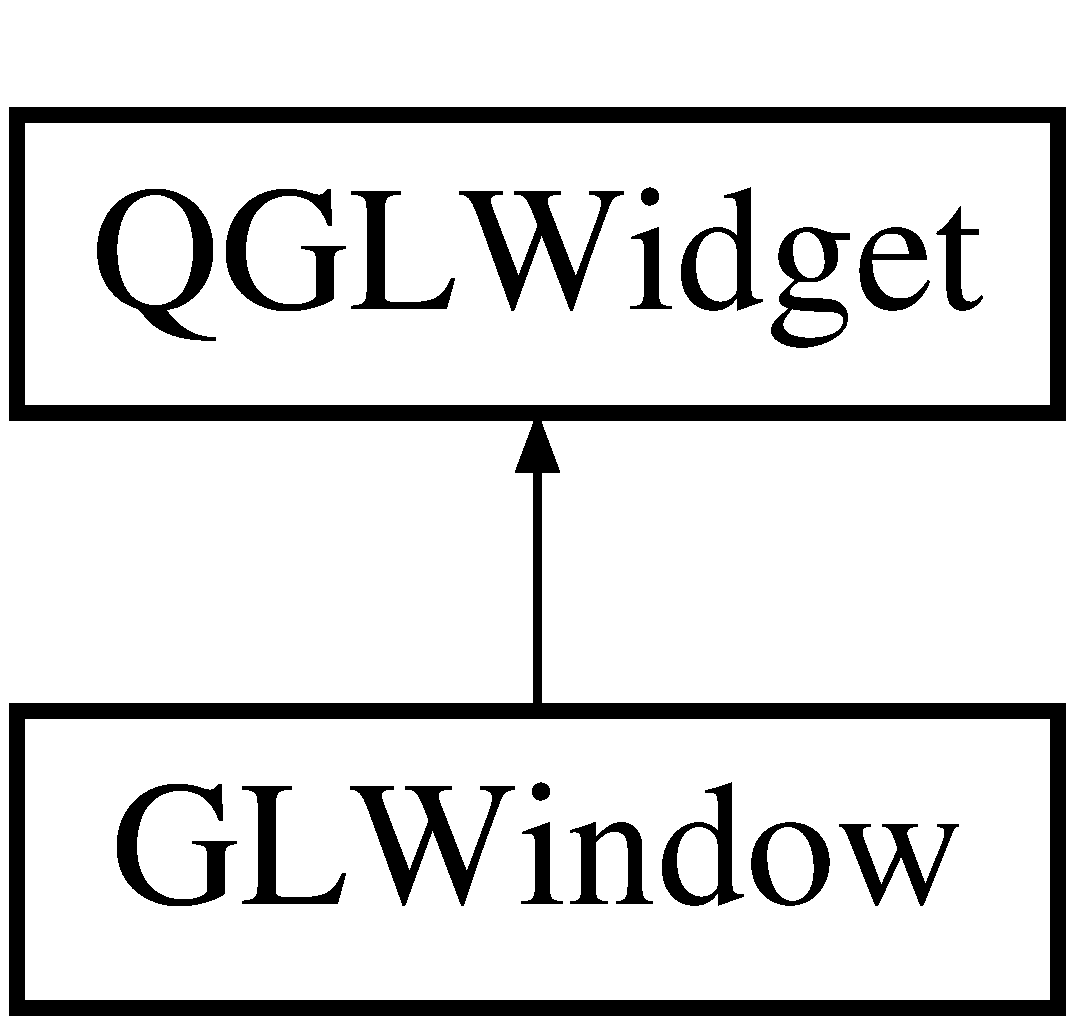
\includegraphics[height=2.000000cm]{class_g_l_window}
\end{center}
\end{figure}
\subsection*{Public Member Functions}
\begin{DoxyCompactItemize}
\item 
\hyperlink{class_g_l_window_a8dfc33113be0a86a53ddbea054f75292}{G\-L\-Window} (Q\-Widget $\ast$\-\_\-parent)
\begin{DoxyCompactList}\small\item\em Constructor for \hyperlink{class_g_l_window}{G\-L\-Window}. \end{DoxyCompactList}\item 
\hypertarget{class_g_l_window_a2eeaea2148f4f72344edd6d1bac9759b}{\hyperlink{class_g_l_window_a2eeaea2148f4f72344edd6d1bac9759b}{$\sim$\-G\-L\-Window} ()}\label{class_g_l_window_a2eeaea2148f4f72344edd6d1bac9759b}

\begin{DoxyCompactList}\small\item\em dtor \end{DoxyCompactList}\item 
\hypertarget{class_g_l_window_ae5d67b7c79c49fac1ee075ec62fa7131}{void {\bfseries toggle\-Animation} ()}\label{class_g_l_window_ae5d67b7c79c49fac1ee075ec62fa7131}

\item 
\hypertarget{class_g_l_window_a72623f17bba6e8b6448efb0572bbdd00}{void {\bfseries process\-Key} (Q\-Key\-Event $\ast$\-\_\-event)}\label{class_g_l_window_a72623f17bba6e8b6448efb0572bbdd00}

\end{DoxyCompactItemize}
\subsection*{Protected Member Functions}
\begin{DoxyCompactItemize}
\item 
\hypertarget{class_g_l_window_a39e39761cd7323806917a217cc7caea5}{void \hyperlink{class_g_l_window_a39e39761cd7323806917a217cc7caea5}{initialize\-G\-L} ()}\label{class_g_l_window_a39e39761cd7323806917a217cc7caea5}

\begin{DoxyCompactList}\small\item\em The following methods must be implimented in the sub class this is called when the window is created. \end{DoxyCompactList}\item 
void \hyperlink{class_g_l_window_abe57c0f40e59cba4c98759121e22eb47}{resize\-G\-L} (const int \-\_\-w, const int \-\_\-h)
\begin{DoxyCompactList}\small\item\em this is called whenever the window is re-\/sized \end{DoxyCompactList}\item 
\hypertarget{class_g_l_window_a9bd2503dd5f812c10a9481f22ecd3403}{void \hyperlink{class_g_l_window_a9bd2503dd5f812c10a9481f22ecd3403}{paint\-G\-L} ()}\label{class_g_l_window_a9bd2503dd5f812c10a9481f22ecd3403}

\begin{DoxyCompactList}\small\item\em this is the main gl drawing routine which is called whenever the window needs to be re-\/drawn \end{DoxyCompactList}\end{DoxyCompactItemize}


\subsection{Detailed Description}
our main glwindow widget for N\-G\-L applications all drawing elements are put in this file 

\subsection{Constructor \& Destructor Documentation}
\hypertarget{class_g_l_window_a8dfc33113be0a86a53ddbea054f75292}{\index{G\-L\-Window@{G\-L\-Window}!G\-L\-Window@{G\-L\-Window}}
\index{G\-L\-Window@{G\-L\-Window}!GLWindow@{G\-L\-Window}}
\subsubsection[{G\-L\-Window}]{\setlength{\rightskip}{0pt plus 5cm}G\-L\-Window\-::\-G\-L\-Window (
\begin{DoxyParamCaption}
\item[{Q\-Widget $\ast$}]{\-\_\-parent}
\end{DoxyParamCaption}
)}}\label{class_g_l_window_a8dfc33113be0a86a53ddbea054f75292}


Constructor for \hyperlink{class_g_l_window}{G\-L\-Window}. 


\begin{DoxyParams}[1]{Parameters}
\mbox{\tt in}  & {\em \-\_\-parent} & the parent window to create the G\-L context in \\
\hline
\end{DoxyParams}


\subsection{Member Function Documentation}
\hypertarget{class_g_l_window_abe57c0f40e59cba4c98759121e22eb47}{\index{G\-L\-Window@{G\-L\-Window}!resize\-G\-L@{resize\-G\-L}}
\index{resize\-G\-L@{resize\-G\-L}!GLWindow@{G\-L\-Window}}
\subsubsection[{resize\-G\-L}]{\setlength{\rightskip}{0pt plus 5cm}void G\-L\-Window\-::resize\-G\-L (
\begin{DoxyParamCaption}
\item[{const int}]{\-\_\-w, }
\item[{const int}]{\-\_\-h}
\end{DoxyParamCaption}
)\hspace{0.3cm}{\ttfamily [protected]}}}\label{class_g_l_window_abe57c0f40e59cba4c98759121e22eb47}


this is called whenever the window is re-\/sized 


\begin{DoxyParams}[1]{Parameters}
\mbox{\tt in}  & {\em \-\_\-w} & the width of the resized window \\
\hline
\mbox{\tt in}  & {\em \-\_\-h} & the height of the resized window \\
\hline
\end{DoxyParams}


The documentation for this class was generated from the following files\-:\begin{DoxyCompactItemize}
\item 
C\-:/\-N\-G\-L/\-Projects/\-Deferred\-Renderer/include/\hyperlink{_g_l_window_8h}{G\-L\-Window.\-h}\item 
C\-:/\-N\-G\-L/\-Projects/\-Deferred\-Renderer/src/G\-L\-Window.\-cpp\end{DoxyCompactItemize}

\hypertarget{classngl_1_1_light}{\section{ngl\-:\-:Light Class Reference}
\label{classngl_1_1_light}\index{ngl\-::\-Light@{ngl\-::\-Light}}
}


Simple class to encapsulate Open\-G\-L \hyperlink{classngl_1_1_light}{Light} functions this will fill in the following structure.  


\subsection*{Public Member Functions}
\begin{DoxyCompactItemize}
\item 
void \hyperlink{classngl_1_1_light_a627f74ab19975d3c63efc1c1750c65f9}{set\-Position} (const Vec3 \&\-\_\-p)
\begin{DoxyCompactList}\small\item\em set the light position \end{DoxyCompactList}\item 
void \hyperlink{classngl_1_1_light_a523bccc4d967748e2ec6bc9c010b3ea6}{set\-Colour} (const Colour \&\-\_\-c)
\begin{DoxyCompactList}\small\item\em set the light colour \end{DoxyCompactList}\item 
void \hyperlink{classngl_1_1_light_a3921ca844ad910bd45e548c696f29aed}{set\-Spec\-Colour} (const Colour \&\-\_\-c)
\begin{DoxyCompactList}\small\item\em set the specular colour \end{DoxyCompactList}\item 
\hypertarget{classngl_1_1_light_a4ef64392703e2ee243ce03ae8a745e9d}{\hyperlink{classngl_1_1_light_a4ef64392703e2ee243ce03ae8a745e9d}{Light} ()}\label{classngl_1_1_light_a4ef64392703e2ee243ce03ae8a745e9d}

\begin{DoxyCompactList}\small\item\em default constructor this set nothing so the light will not illuminate \end{DoxyCompactList}\item 
\hypertarget{classngl_1_1_light_a775bed44aff46ab92a463e7b0d409564}{\hyperlink{classngl_1_1_light_a775bed44aff46ab92a463e7b0d409564}{Light} (const \hyperlink{classngl_1_1_light}{Light} \&\-\_\-l)}\label{classngl_1_1_light_a775bed44aff46ab92a463e7b0d409564}

\begin{DoxyCompactList}\small\item\em copy ctor this set nothing so the light will not illuminate \end{DoxyCompactList}\item 
\hyperlink{classngl_1_1_light_a1a39ba791902f538c44c8f78f92083f5}{Light} (const Vec3 \&\-\_\-pos, const Colour \&\-\_\-col, L\-I\-G\-H\-T\-M\-O\-D\-E\-S \-\_\-lightmode)
\begin{DoxyCompactList}\small\item\em ctor to create the light \end{DoxyCompactList}\item 
\hyperlink{classngl_1_1_light_a64a48426b9821ef040efb0928fd27414}{Light} (const Vec3 \&\-\_\-pos, const Colour \&\-\_\-col, const Colour \&\-\_\-spec\-Colour, L\-I\-G\-H\-T\-M\-O\-D\-E\-S \-\_\-lightmode)
\begin{DoxyCompactList}\small\item\em ctor to create the light \end{DoxyCompactList}\item 
\hypertarget{classngl_1_1_light_a3a304983c33a2ed286299e34d8089d02}{virtual \hyperlink{classngl_1_1_light_a3a304983c33a2ed286299e34d8089d02}{$\sim$\-Light} ()}\label{classngl_1_1_light_a3a304983c33a2ed286299e34d8089d02}

\begin{DoxyCompactList}\small\item\em destructor when light is destroyed we turn it off \end{DoxyCompactList}\item 
\hypertarget{classngl_1_1_light_ad8a265e7c2076ad1c7d24fefd4201df0}{void \hyperlink{classngl_1_1_light_ad8a265e7c2076ad1c7d24fefd4201df0}{disable} ()}\label{classngl_1_1_light_ad8a265e7c2076ad1c7d24fefd4201df0}

\begin{DoxyCompactList}\small\item\em Disable the light by calling gl\-Disable(G\-L\-\_\-\-L\-I\-G\-H\-T0+\-Light\-No);. \end{DoxyCompactList}\item 
virtual void \hyperlink{classngl_1_1_light_a1fa84fda6ad283674a351aa0fdc7d12a}{enable} ()
\begin{DoxyCompactList}\small\item\em Enables the light and automatically allocates an Open\-G\-L light I\-D. \end{DoxyCompactList}\item 
\hypertarget{classngl_1_1_light_a328389a585ba1efcf6eb08fd5b7b0181}{void \hyperlink{classngl_1_1_light_a328389a585ba1efcf6eb08fd5b7b0181}{show} ()}\label{classngl_1_1_light_a328389a585ba1efcf6eb08fd5b7b0181}

\begin{DoxyCompactList}\small\item\em displays the light in the scene \end{DoxyCompactList}\item 
Vec4 \& \hyperlink{classngl_1_1_light_a57a8c683f7db93d059a4a2467ac3e980}{get\-Pos} ()
\begin{DoxyCompactList}\small\item\em returns the current light position as a Vector \end{DoxyCompactList}\item 
Colour \& \hyperlink{classngl_1_1_light_a8d3daa5594e73456cae3555aac07136d}{get\-Colour} ()
\begin{DoxyCompactList}\small\item\em returns the current light colour \end{DoxyCompactList}\item 
Colour \& \hyperlink{classngl_1_1_light_ac7438a00c9bca8655dce924a338d93c6}{get\-Spec\-Colour} ()
\begin{DoxyCompactList}\small\item\em returns the current light Specular colour \end{DoxyCompactList}\item 
void \hyperlink{classngl_1_1_light_afb7b9d8db15a4fd4e923049946e71681}{set\-Attenuation} (Real \-\_\-constant=1.\-0, Real \-\_\-linear=0.\-0, Real \-\_\-quadratic=0.\-0)
\begin{DoxyCompactList}\small\item\em set the light attenuation \end{DoxyCompactList}\item 
void \hyperlink{classngl_1_1_light_a7bc1c8e03bf7647364474b346ec37a09}{write\-X\-M\-L} (Q\-Xml\-Stream\-Writer $\ast$\-\_\-stream, const std\-::string \-\_\-tag=\char`\"{}Light\char`\"{}) const 
\begin{DoxyCompactList}\small\item\em write class to xml stream \end{DoxyCompactList}\item 
void \hyperlink{classngl_1_1_light_a2f082480063a6b066864d4d0f056e4f1}{load\-To\-Shader} (std\-::string \-\_\-uniform\-Name) const 
\begin{DoxyCompactList}\small\item\em method to load the current light values to the shader that is active at present \end{DoxyCompactList}\item 
void \hyperlink{classngl_1_1_light_a329aacaa1907e39a44c7bcbd3d4ae0aa}{set\-Transform} (ngl\-::\-Mat4 \&\-\_\-t)
\begin{DoxyCompactList}\small\item\em set a transform so that the light position is multiplied by this value (default is identity matrix) \end{DoxyCompactList}\end{DoxyCompactItemize}
\subsection*{Protected Attributes}
\begin{DoxyCompactItemize}
\item 
\hypertarget{classngl_1_1_light_afe8a51aeb598b51b3c42a6ecddd38d08}{Vec4 \hyperlink{classngl_1_1_light_afe8a51aeb598b51b3c42a6ecddd38d08}{m\-\_\-position}}\label{classngl_1_1_light_afe8a51aeb598b51b3c42a6ecddd38d08}

\begin{DoxyCompactList}\small\item\em m\-\_\-pos is used to store the light position w used for point / dir light values \end{DoxyCompactList}\item 
\hypertarget{classngl_1_1_light_a7bc1cdc3603b217e66bf4e1d9b1b8e8c}{Colour \hyperlink{classngl_1_1_light_a7bc1cdc3603b217e66bf4e1d9b1b8e8c}{m\-\_\-diffuse}}\label{classngl_1_1_light_a7bc1cdc3603b217e66bf4e1d9b1b8e8c}

\begin{DoxyCompactList}\small\item\em Colour used to give the light a colour. \end{DoxyCompactList}\item 
\hypertarget{classngl_1_1_light_aa12f58491b9237345930721b5ac94932}{Colour \hyperlink{classngl_1_1_light_aa12f58491b9237345930721b5ac94932}{m\-\_\-specular}}\label{classngl_1_1_light_aa12f58491b9237345930721b5ac94932}

\begin{DoxyCompactList}\small\item\em specular highlight colour used for the lights \end{DoxyCompactList}\item 
\hypertarget{classngl_1_1_light_acc8c0099d1b3437bc814d19de9d5025f}{Colour \hyperlink{classngl_1_1_light_acc8c0099d1b3437bc814d19de9d5025f}{m\-\_\-ambient}}\label{classngl_1_1_light_acc8c0099d1b3437bc814d19de9d5025f}

\begin{DoxyCompactList}\small\item\em ambient light colour used for the lights \end{DoxyCompactList}\item 
\hypertarget{classngl_1_1_light_acea764757d046277f3dc5d3f4adf5597}{L\-I\-G\-H\-T\-M\-O\-D\-E\-S \hyperlink{classngl_1_1_light_acea764757d046277f3dc5d3f4adf5597}{m\-\_\-light\-Mode}}\label{classngl_1_1_light_acea764757d046277f3dc5d3f4adf5597}

\begin{DoxyCompactList}\small\item\em used to hold the current lights mode \end{DoxyCompactList}\item 
\hypertarget{classngl_1_1_light_ae599f2dfec737b23af75cbcb6be6613e}{Real \hyperlink{classngl_1_1_light_ae599f2dfec737b23af75cbcb6be6613e}{m\-\_\-constant\-Atten}}\label{classngl_1_1_light_ae599f2dfec737b23af75cbcb6be6613e}

\begin{DoxyCompactList}\small\item\em attenuation value for constant falloff \end{DoxyCompactList}\item 
\hypertarget{classngl_1_1_light_aebe8996368d8c7598cffba36883084e0}{Real \hyperlink{classngl_1_1_light_aebe8996368d8c7598cffba36883084e0}{m\-\_\-linear\-Atten}}\label{classngl_1_1_light_aebe8996368d8c7598cffba36883084e0}

\begin{DoxyCompactList}\small\item\em attenuation value for linear falloff \end{DoxyCompactList}\item 
\hypertarget{classngl_1_1_light_a926e5c7567ad0b2e09548dd6a8e60d7c}{Real \hyperlink{classngl_1_1_light_a926e5c7567ad0b2e09548dd6a8e60d7c}{m\-\_\-quadratic\-Atten}}\label{classngl_1_1_light_a926e5c7567ad0b2e09548dd6a8e60d7c}

\begin{DoxyCompactList}\small\item\em attenuation value for Quadratic falloff \end{DoxyCompactList}\item 
\hypertarget{classngl_1_1_light_a1cdd46b20e1d7f6e8d4aa01a4b3f72ad}{Real \hyperlink{classngl_1_1_light_a1cdd46b20e1d7f6e8d4aa01a4b3f72ad}{m\-\_\-active}}\label{classngl_1_1_light_a1cdd46b20e1d7f6e8d4aa01a4b3f72ad}

\begin{DoxyCompactList}\small\item\em active if true else off \end{DoxyCompactList}\item 
\hypertarget{classngl_1_1_light_a61ea1115270a6b4798a6383a8c2c1b26}{Real \hyperlink{classngl_1_1_light_a61ea1115270a6b4798a6383a8c2c1b26}{m\-\_\-cutoff\-Angle}}\label{classngl_1_1_light_a61ea1115270a6b4798a6383a8c2c1b26}

\begin{DoxyCompactList}\small\item\em the spot cutoff angle for directional and point lights this is set to 180 by default, and other values are cos(radians(angle)) \end{DoxyCompactList}\item 
\hypertarget{classngl_1_1_light_ab905d7f0ee91e2a482ce5d4d99bb81fd}{ngl\-::\-Mat4 \hyperlink{classngl_1_1_light_ab905d7f0ee91e2a482ce5d4d99bb81fd}{m\-\_\-transform}}\label{classngl_1_1_light_ab905d7f0ee91e2a482ce5d4d99bb81fd}

\begin{DoxyCompactList}\small\item\em the transform applied to the light before loading to the shader this is usually the inverse projection matrix for normal Open\-G\-L style eye-\/cord calculations but is left for the Application to calculate and pass for easier implementation of different light models \end{DoxyCompactList}\end{DoxyCompactItemize}


\subsection{Detailed Description}
Simple class to encapsulate Open\-G\-L \hyperlink{classngl_1_1_light}{Light} functions this will fill in the following structure. 

struct Lights \{ vec4 position; vec4 ambient; vec4 diffuse; vec4 specular; \}; \begin{DoxyAuthor}{Author}
Jon Macey 
\end{DoxyAuthor}
\begin{DoxyVersion}{Version}
5.\-0 
\end{DoxyVersion}
\begin{DoxyDate}{Date}
18/08/11 updated to remove deprecated G\-L stuff and all work with glsl 150 Last Revision 29/10/09 Updated to N\-C\-C\-A coding standard 
\end{DoxyDate}
\begin{DoxyRefDesc}{Todo}
\item[\hyperlink{todo__todo000003}{Todo}]this will need to be changed to work with G\-L\-S\-L lights for G\-L\-\_\-\-V\-E\-R\-S\-I\-O\-N $>$ 3.\-x \end{DoxyRefDesc}


\subsection{Constructor \& Destructor Documentation}
\hypertarget{classngl_1_1_light_a1a39ba791902f538c44c8f78f92083f5}{\index{ngl\-::\-Light@{ngl\-::\-Light}!Light@{Light}}
\index{Light@{Light}!ngl::Light@{ngl\-::\-Light}}
\subsubsection[{Light}]{\setlength{\rightskip}{0pt plus 5cm}ngl\-::\-Light\-::\-Light (
\begin{DoxyParamCaption}
\item[{const Vec3 \&}]{\-\_\-pos, }
\item[{const Colour \&}]{\-\_\-col, }
\item[{L\-I\-G\-H\-T\-M\-O\-D\-E\-S}]{\-\_\-lightmode}
\end{DoxyParamCaption}
)}}\label{classngl_1_1_light_a1a39ba791902f538c44c8f78f92083f5}


ctor to create the light 


\begin{DoxyParams}[1]{Parameters}
\mbox{\tt in}  & {\em \-\_\-pos} & the light position \\
\hline
\mbox{\tt in}  & {\em \-\_\-col} & the light colour \\
\hline
\mbox{\tt in}  & {\em \-\_\-lightmode} & the mode to set the light to either local or remote \\
\hline
\end{DoxyParams}
\hypertarget{classngl_1_1_light_a64a48426b9821ef040efb0928fd27414}{\index{ngl\-::\-Light@{ngl\-::\-Light}!Light@{Light}}
\index{Light@{Light}!ngl::Light@{ngl\-::\-Light}}
\subsubsection[{Light}]{\setlength{\rightskip}{0pt plus 5cm}ngl\-::\-Light\-::\-Light (
\begin{DoxyParamCaption}
\item[{const Vec3 \&}]{\-\_\-pos, }
\item[{const Colour \&}]{\-\_\-col, }
\item[{const Colour \&}]{\-\_\-spec\-Colour, }
\item[{L\-I\-G\-H\-T\-M\-O\-D\-E\-S}]{\-\_\-lightmode}
\end{DoxyParamCaption}
)}}\label{classngl_1_1_light_a64a48426b9821ef040efb0928fd27414}


ctor to create the light 


\begin{DoxyParams}[1]{Parameters}
\mbox{\tt in}  & {\em \-\_\-pos} & the light position \\
\hline
\mbox{\tt in}  & {\em \-\_\-col} & the light colour \\
\hline
\mbox{\tt in}  & {\em \-\_\-spec\-Colour} & the specular component of the light \\
\hline
\mbox{\tt in}  & {\em \-\_\-lightmode} & the mode to set the light to either local or remote \\
\hline
\end{DoxyParams}


\subsection{Member Function Documentation}
\hypertarget{classngl_1_1_light_a1fa84fda6ad283674a351aa0fdc7d12a}{\index{ngl\-::\-Light@{ngl\-::\-Light}!enable@{enable}}
\index{enable@{enable}!ngl::Light@{ngl\-::\-Light}}
\subsubsection[{enable}]{\setlength{\rightskip}{0pt plus 5cm}virtual void ngl\-::\-Light\-::enable (
\begin{DoxyParamCaption}
{}
\end{DoxyParamCaption}
)\hspace{0.3cm}{\ttfamily [virtual]}}}\label{classngl_1_1_light_a1fa84fda6ad283674a351aa0fdc7d12a}


Enables the light and automatically allocates an Open\-G\-L light I\-D. 

\begin{DoxyReturn}{Returns}
true if there is a free open\-G\-L light I\-D available. 
\end{DoxyReturn}
\hypertarget{classngl_1_1_light_a8d3daa5594e73456cae3555aac07136d}{\index{ngl\-::\-Light@{ngl\-::\-Light}!get\-Colour@{get\-Colour}}
\index{get\-Colour@{get\-Colour}!ngl::Light@{ngl\-::\-Light}}
\subsubsection[{get\-Colour}]{\setlength{\rightskip}{0pt plus 5cm}Colour\& ngl\-::\-Light\-::get\-Colour (
\begin{DoxyParamCaption}
{}
\end{DoxyParamCaption}
)\hspace{0.3cm}{\ttfamily [inline]}}}\label{classngl_1_1_light_a8d3daa5594e73456cae3555aac07136d}


returns the current light colour 

\begin{DoxyReturn}{Returns}
Colour colour 
\end{DoxyReturn}
\hypertarget{classngl_1_1_light_a57a8c683f7db93d059a4a2467ac3e980}{\index{ngl\-::\-Light@{ngl\-::\-Light}!get\-Pos@{get\-Pos}}
\index{get\-Pos@{get\-Pos}!ngl::Light@{ngl\-::\-Light}}
\subsubsection[{get\-Pos}]{\setlength{\rightskip}{0pt plus 5cm}Vec4\& ngl\-::\-Light\-::get\-Pos (
\begin{DoxyParamCaption}
{}
\end{DoxyParamCaption}
)\hspace{0.3cm}{\ttfamily [inline]}}}\label{classngl_1_1_light_a57a8c683f7db93d059a4a2467ac3e980}


returns the current light position as a Vector 

\begin{DoxyReturn}{Returns}
Vector pos 
\end{DoxyReturn}
\hypertarget{classngl_1_1_light_ac7438a00c9bca8655dce924a338d93c6}{\index{ngl\-::\-Light@{ngl\-::\-Light}!get\-Spec\-Colour@{get\-Spec\-Colour}}
\index{get\-Spec\-Colour@{get\-Spec\-Colour}!ngl::Light@{ngl\-::\-Light}}
\subsubsection[{get\-Spec\-Colour}]{\setlength{\rightskip}{0pt plus 5cm}Colour\& ngl\-::\-Light\-::get\-Spec\-Colour (
\begin{DoxyParamCaption}
{}
\end{DoxyParamCaption}
)\hspace{0.3cm}{\ttfamily [inline]}}}\label{classngl_1_1_light_ac7438a00c9bca8655dce924a338d93c6}


returns the current light Specular colour 

\begin{DoxyReturn}{Returns}
Colour Spec colour 
\end{DoxyReturn}
\hypertarget{classngl_1_1_light_a2f082480063a6b066864d4d0f056e4f1}{\index{ngl\-::\-Light@{ngl\-::\-Light}!load\-To\-Shader@{load\-To\-Shader}}
\index{load\-To\-Shader@{load\-To\-Shader}!ngl::Light@{ngl\-::\-Light}}
\subsubsection[{load\-To\-Shader}]{\setlength{\rightskip}{0pt plus 5cm}void ngl\-::\-Light\-::load\-To\-Shader (
\begin{DoxyParamCaption}
\item[{std\-::string}]{\-\_\-uniform\-Name}
\end{DoxyParamCaption}
) const}}\label{classngl_1_1_light_a2f082480063a6b066864d4d0f056e4f1}


method to load the current light values to the shader that is active at present 


\begin{DoxyParams}[1]{Parameters}
\mbox{\tt in}  & {\em \-\_\-uniform\-Name} & name of the uniform to set \\
\hline
\end{DoxyParams}
\hypertarget{classngl_1_1_light_afb7b9d8db15a4fd4e923049946e71681}{\index{ngl\-::\-Light@{ngl\-::\-Light}!set\-Attenuation@{set\-Attenuation}}
\index{set\-Attenuation@{set\-Attenuation}!ngl::Light@{ngl\-::\-Light}}
\subsubsection[{set\-Attenuation}]{\setlength{\rightskip}{0pt plus 5cm}void ngl\-::\-Light\-::set\-Attenuation (
\begin{DoxyParamCaption}
\item[{Real}]{\-\_\-constant = {\ttfamily 1.0}, }
\item[{Real}]{\-\_\-linear = {\ttfamily 0.0}, }
\item[{Real}]{\-\_\-quadratic = {\ttfamily 0.0}}
\end{DoxyParamCaption}
)}}\label{classngl_1_1_light_afb7b9d8db15a4fd4e923049946e71681}


set the light attenuation 


\begin{DoxyParams}[1]{Parameters}
\mbox{\tt in}  & {\em \-\_\-constant} & the constant attenuation \\
\hline
\mbox{\tt in}  & {\em \-\_\-linear} & attenuation \\
\hline
\mbox{\tt in}  & {\em \-\_\-quadratic} & attenuation \\
\hline
\end{DoxyParams}
\hypertarget{classngl_1_1_light_a523bccc4d967748e2ec6bc9c010b3ea6}{\index{ngl\-::\-Light@{ngl\-::\-Light}!set\-Colour@{set\-Colour}}
\index{set\-Colour@{set\-Colour}!ngl::Light@{ngl\-::\-Light}}
\subsubsection[{set\-Colour}]{\setlength{\rightskip}{0pt plus 5cm}void ngl\-::\-Light\-::set\-Colour (
\begin{DoxyParamCaption}
\item[{const Colour \&}]{\-\_\-c}
\end{DoxyParamCaption}
)\hspace{0.3cm}{\ttfamily [inline]}}}\label{classngl_1_1_light_a523bccc4d967748e2ec6bc9c010b3ea6}


set the light colour 


\begin{DoxyParams}[1]{Parameters}
\mbox{\tt in}  & {\em \-\_\-c} & the colour to set \\
\hline
\end{DoxyParams}
\hypertarget{classngl_1_1_light_a627f74ab19975d3c63efc1c1750c65f9}{\index{ngl\-::\-Light@{ngl\-::\-Light}!set\-Position@{set\-Position}}
\index{set\-Position@{set\-Position}!ngl::Light@{ngl\-::\-Light}}
\subsubsection[{set\-Position}]{\setlength{\rightskip}{0pt plus 5cm}void ngl\-::\-Light\-::set\-Position (
\begin{DoxyParamCaption}
\item[{const Vec3 \&}]{\-\_\-p}
\end{DoxyParamCaption}
)\hspace{0.3cm}{\ttfamily [inline]}}}\label{classngl_1_1_light_a627f74ab19975d3c63efc1c1750c65f9}


set the light position 


\begin{DoxyParams}[1]{Parameters}
\mbox{\tt in}  & {\em \-\_\-p} & the new light position \\
\hline
\end{DoxyParams}
\hypertarget{classngl_1_1_light_a3921ca844ad910bd45e548c696f29aed}{\index{ngl\-::\-Light@{ngl\-::\-Light}!set\-Spec\-Colour@{set\-Spec\-Colour}}
\index{set\-Spec\-Colour@{set\-Spec\-Colour}!ngl::Light@{ngl\-::\-Light}}
\subsubsection[{set\-Spec\-Colour}]{\setlength{\rightskip}{0pt plus 5cm}void ngl\-::\-Light\-::set\-Spec\-Colour (
\begin{DoxyParamCaption}
\item[{const Colour \&}]{\-\_\-c}
\end{DoxyParamCaption}
)\hspace{0.3cm}{\ttfamily [inline]}}}\label{classngl_1_1_light_a3921ca844ad910bd45e548c696f29aed}


set the specular colour 


\begin{DoxyParams}[1]{Parameters}
\mbox{\tt in}  & {\em \-\_\-c} & the colour to set for the specular \\
\hline
\end{DoxyParams}
\hypertarget{classngl_1_1_light_a329aacaa1907e39a44c7bcbd3d4ae0aa}{\index{ngl\-::\-Light@{ngl\-::\-Light}!set\-Transform@{set\-Transform}}
\index{set\-Transform@{set\-Transform}!ngl::Light@{ngl\-::\-Light}}
\subsubsection[{set\-Transform}]{\setlength{\rightskip}{0pt plus 5cm}void ngl\-::\-Light\-::set\-Transform (
\begin{DoxyParamCaption}
\item[{ngl\-::\-Mat4 \&}]{\-\_\-t}
\end{DoxyParamCaption}
)}}\label{classngl_1_1_light_a329aacaa1907e39a44c7bcbd3d4ae0aa}


set a transform so that the light position is multiplied by this value (default is identity matrix) 


\begin{DoxyParams}[1]{Parameters}
\mbox{\tt in}  & {\em \-\_\-t} & the transform matrix \\
\hline
\end{DoxyParams}
\hypertarget{classngl_1_1_light_a7bc1c8e03bf7647364474b346ec37a09}{\index{ngl\-::\-Light@{ngl\-::\-Light}!write\-X\-M\-L@{write\-X\-M\-L}}
\index{write\-X\-M\-L@{write\-X\-M\-L}!ngl::Light@{ngl\-::\-Light}}
\subsubsection[{write\-X\-M\-L}]{\setlength{\rightskip}{0pt plus 5cm}void ngl\-::\-Light\-::write\-X\-M\-L (
\begin{DoxyParamCaption}
\item[{Q\-Xml\-Stream\-Writer $\ast$}]{\-\_\-stream, }
\item[{const std\-::string}]{\-\_\-tag = {\ttfamily \char`\"{}Light\char`\"{}}}
\end{DoxyParamCaption}
) const}}\label{classngl_1_1_light_a7bc1c8e03bf7647364474b346ec37a09}


write class to xml stream 


\begin{DoxyParams}[1]{Parameters}
\mbox{\tt in}  & {\em \-\_\-stream} & the xml stream to write to \\
\hline
\mbox{\tt in}  & {\em \-\_\-name} & an overidable token name for the xml tag \\
\hline
\end{DoxyParams}


The documentation for this class was generated from the following file\-:\begin{DoxyCompactItemize}
\item 
C\-:/\-N\-G\-L/\-Projects/\-Deferred\-Renderer/include/ngl/\hyperlink{_light_8h}{Light.\-h}\end{DoxyCompactItemize}

\hypertarget{class_main_window}{\section{Main\-Window Class Reference}
\label{class_main_window}\index{Main\-Window@{Main\-Window}}
}


the main re-\/sizable window which contains a \hyperlink{class_g_l_window}{G\-L\-Window} widget used to hold our basic gl applications  




{\ttfamily \#include $<$Main\-Window.\-h$>$}

Inheritance diagram for Main\-Window\-:\begin{figure}[H]
\begin{center}
\leavevmode
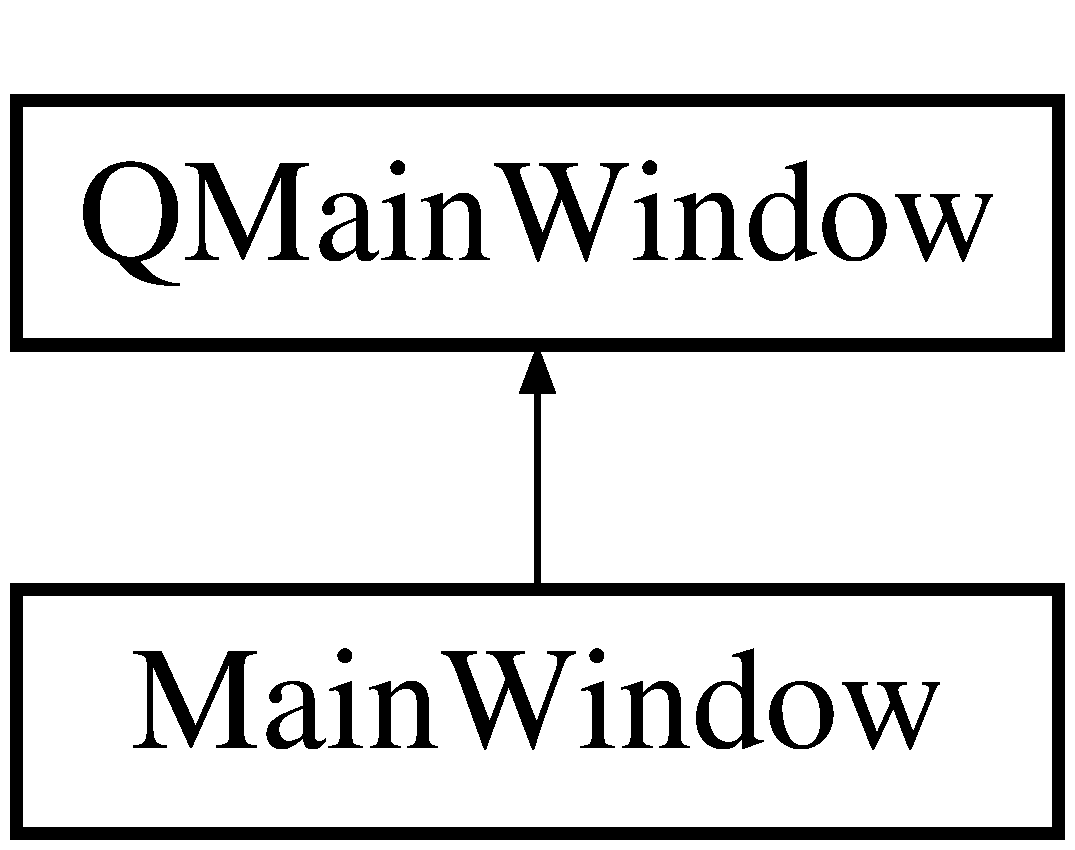
\includegraphics[height=2.000000cm]{class_main_window}
\end{center}
\end{figure}
\subsection*{Public Member Functions}
\begin{DoxyCompactItemize}
\item 
\hyperlink{class_main_window_a93cfdcac35db98baf6a7d2c2738a2006}{Main\-Window} (Q\-Widget $\ast$\-\_\-parent=0)
\begin{DoxyCompactList}\small\item\em constructor \end{DoxyCompactList}\item 
\hypertarget{class_main_window_ae98d00a93bc118200eeef9f9bba1dba7}{\hyperlink{class_main_window_ae98d00a93bc118200eeef9f9bba1dba7}{$\sim$\-Main\-Window} ()}\label{class_main_window_ae98d00a93bc118200eeef9f9bba1dba7}

\begin{DoxyCompactList}\small\item\em dtor free up the \hyperlink{class_g_l_window}{G\-L\-Window} and all resources \end{DoxyCompactList}\end{DoxyCompactItemize}
\subsection*{Protected Member Functions}
\begin{DoxyCompactItemize}
\item 
void \hyperlink{class_main_window_a3c2e352934c6318d405c3d2b0e07729c}{key\-Press\-Event} (Q\-Key\-Event $\ast$\-\_\-event)
\begin{DoxyCompactList}\small\item\em override the key\-Press\-Event inherited from Q\-Object so we can handle key presses. \end{DoxyCompactList}\item 
void \hyperlink{class_main_window_a8ed35ee3d9b815ed32c11d1e13957503}{resize\-Event} (Q\-Resize\-Event $\ast$\-\_\-event)
\begin{DoxyCompactList}\small\item\em override the resize\-Event inherited from Q\-Object so we can handle key presses. \end{DoxyCompactList}\end{DoxyCompactItemize}


\subsection{Detailed Description}
the main re-\/sizable window which contains a \hyperlink{class_g_l_window}{G\-L\-Window} widget used to hold our basic gl applications 

\subsection{Constructor \& Destructor Documentation}
\hypertarget{class_main_window_a93cfdcac35db98baf6a7d2c2738a2006}{\index{Main\-Window@{Main\-Window}!Main\-Window@{Main\-Window}}
\index{Main\-Window@{Main\-Window}!MainWindow@{Main\-Window}}
\subsubsection[{Main\-Window}]{\setlength{\rightskip}{0pt plus 5cm}Main\-Window\-::\-Main\-Window (
\begin{DoxyParamCaption}
\item[{Q\-Widget $\ast$}]{\-\_\-parent = {\ttfamily 0}}
\end{DoxyParamCaption}
)}}\label{class_main_window_a93cfdcac35db98baf6a7d2c2738a2006}


constructor 


\begin{DoxyParams}{Parameters}
{\em \-\_\-parent} & the parent window the for this window \\
\hline
\end{DoxyParams}


\subsection{Member Function Documentation}
\hypertarget{class_main_window_a3c2e352934c6318d405c3d2b0e07729c}{\index{Main\-Window@{Main\-Window}!key\-Press\-Event@{key\-Press\-Event}}
\index{key\-Press\-Event@{key\-Press\-Event}!MainWindow@{Main\-Window}}
\subsubsection[{key\-Press\-Event}]{\setlength{\rightskip}{0pt plus 5cm}void Main\-Window\-::key\-Press\-Event (
\begin{DoxyParamCaption}
\item[{Q\-Key\-Event $\ast$}]{\-\_\-event}
\end{DoxyParamCaption}
)\hspace{0.3cm}{\ttfamily [protected]}}}\label{class_main_window_a3c2e352934c6318d405c3d2b0e07729c}


override the key\-Press\-Event inherited from Q\-Object so we can handle key presses. 


\begin{DoxyParams}[1]{Parameters}
\mbox{\tt in}  & {\em \-\_\-event} & the event to process \\
\hline
\end{DoxyParams}
\hypertarget{class_main_window_a8ed35ee3d9b815ed32c11d1e13957503}{\index{Main\-Window@{Main\-Window}!resize\-Event@{resize\-Event}}
\index{resize\-Event@{resize\-Event}!MainWindow@{Main\-Window}}
\subsubsection[{resize\-Event}]{\setlength{\rightskip}{0pt plus 5cm}void Main\-Window\-::resize\-Event (
\begin{DoxyParamCaption}
\item[{Q\-Resize\-Event $\ast$}]{\-\_\-event}
\end{DoxyParamCaption}
)\hspace{0.3cm}{\ttfamily [protected]}}}\label{class_main_window_a8ed35ee3d9b815ed32c11d1e13957503}


override the resize\-Event inherited from Q\-Object so we can handle key presses. 


\begin{DoxyParams}[1]{Parameters}
\mbox{\tt in}  & {\em \-\_\-event} & the event to process \\
\hline
\end{DoxyParams}


The documentation for this class was generated from the following files\-:\begin{DoxyCompactItemize}
\item 
C\-:/\-N\-G\-L/\-Projects/\-Deferred\-Renderer/include/\hyperlink{_main_window_8h}{Main\-Window.\-h}\item 
C\-:/\-N\-G\-L/\-Projects/\-Deferred\-Renderer/src/Main\-Window.\-cpp\end{DoxyCompactItemize}

\hypertarget{class_object_loader}{\section{Object\-Loader Class Reference}
\label{class_object_loader}\index{Object\-Loader@{Object\-Loader}}
}
\subsection*{Public Member Functions}
\begin{DoxyCompactItemize}
\item 
\hypertarget{class_object_loader_ac28a22d6234864b00d3078bc1676a852}{\hyperlink{class_object_loader_ac28a22d6234864b00d3078bc1676a852}{Object\-Loader} (const std\-::string \-\_\-shader\-Program\-Name, const std\-::string \-\_\-vertex\-Shader\-File\-Name, const std\-::string \-\_\-fragment\-Shader\-Filename)}\label{class_object_loader_ac28a22d6234864b00d3078bc1676a852}

\begin{DoxyCompactList}\small\item\em ctor for loading model and attached textures and shaders. It creates the shader \end{DoxyCompactList}\item 
\hypertarget{class_object_loader_ac2397df02e74d50980604991fb772585}{\hyperlink{class_object_loader_ac2397df02e74d50980604991fb772585}{Object\-Loader} (const std\-::string \-\_\-shader\-Program\-Name)}\label{class_object_loader_ac2397df02e74d50980604991fb772585}

\begin{DoxyCompactList}\small\item\em ctor for loading model and textures using shaders that already exist. It uses an existing shader \end{DoxyCompactList}\item 
\hypertarget{class_object_loader_abe35e670f22d62f56a95e28b67b43c93}{\hyperlink{class_object_loader_abe35e670f22d62f56a95e28b67b43c93}{$\sim$\-Object\-Loader} ()}\label{class_object_loader_abe35e670f22d62f56a95e28b67b43c93}

\begin{DoxyCompactList}\small\item\em dctor \end{DoxyCompactList}\item 
\hypertarget{class_object_loader_a13165ae8f1c06aa6d2e42a25cce1ccbe}{G\-Luint {\bfseries get\-Shader\-Program\-Handle} () const }\label{class_object_loader_a13165ae8f1c06aa6d2e42a25cce1ccbe}

\item 
\hypertarget{class_object_loader_a1545820e46bc97530d34454b2bfe7b20}{void \hyperlink{class_object_loader_a1545820e46bc97530d34454b2bfe7b20}{set\-Shader\-As\-Active} () const }\label{class_object_loader_a1545820e46bc97530d34454b2bfe7b20}

\begin{DoxyCompactList}\small\item\em Set the current shader as the active one. All the information sent to the shader will be on this one. \end{DoxyCompactList}\item 
\hypertarget{class_object_loader_a0e17d739447bc8b758f7d0826ff0d82e}{void \hyperlink{class_object_loader_a0e17d739447bc8b758f7d0826ff0d82e}{load\-Mesh} (const std\-::string \-\_\-mesh\-File\-Name)}\label{class_object_loader_a0e17d739447bc8b758f7d0826ff0d82e}

\begin{DoxyCompactList}\small\item\em loads a Mesh, O\-B\-J file. Method not tested yet. \end{DoxyCompactList}\item 
\hypertarget{class_object_loader_ab1680ee5acad9c8a02ff7b87460c9d30}{void \hyperlink{class_object_loader_ab1680ee5acad9c8a02ff7b87460c9d30}{load\-Texture} (const std\-::string \-\_\-texture\-File\-Name)}\label{class_object_loader_ab1680ee5acad9c8a02ff7b87460c9d30}

\begin{DoxyCompactList}\small\item\em loads a texture file. Method not tested yet. \end{DoxyCompactList}\end{DoxyCompactItemize}
\subsection*{Public Attributes}
\begin{DoxyCompactItemize}
\item 
\hypertarget{class_object_loader_a477c658216ae723c06ffefb1cc123a04}{G\-Lint \hyperlink{class_object_loader_a477c658216ae723c06ffefb1cc123a04}{m\-\_\-texture\-Index}}\label{class_object_loader_a477c658216ae723c06ffefb1cc123a04}

\begin{DoxyCompactList}\small\item\em Index for counting textures loaded and used by this shader. \end{DoxyCompactList}\item 
\hypertarget{class_object_loader_a25b0c1c8390e13a351ab7334fc1dc1fc}{bool {\bfseries m\-\_\-mesh\-Is\-Loaded}}\label{class_object_loader_a25b0c1c8390e13a351ab7334fc1dc1fc}

\item 
\hypertarget{class_object_loader_a3d70ee2ce56daeaced002dd6d3797283}{std\-::vector$<$ \hyperlink{classngl_1_1_light}{ngl\-::\-Light} $\ast$ $>$ \hyperlink{class_object_loader_a3d70ee2ce56daeaced002dd6d3797283}{m\-\_\-light}}\label{class_object_loader_a3d70ee2ce56daeaced002dd6d3797283}

\begin{DoxyCompactList}\small\item\em vector containing all the point lights in the scene \end{DoxyCompactList}\item 
\hypertarget{class_object_loader_a759ade5adb03d58bca0ff4b966994081}{std\-::vector$<$ \hyperlink{class_spotlight}{Spotlight} $\ast$ $>$ \hyperlink{class_object_loader_a759ade5adb03d58bca0ff4b966994081}{m\-\_\-spotlight}}\label{class_object_loader_a759ade5adb03d58bca0ff4b966994081}

\begin{DoxyCompactList}\small\item\em vector containing all the point lights in the scene \end{DoxyCompactList}\item 
\hypertarget{class_object_loader_a2ea656821677e535f3e0044536c55c9f}{std\-::vector$<$ ngl\-::\-L\-I\-G\-H\-T\-M\-O\-D\-E\-S $>$ \hyperlink{class_object_loader_a2ea656821677e535f3e0044536c55c9f}{m\-\_\-light\-Type}}\label{class_object_loader_a2ea656821677e535f3e0044536c55c9f}

\begin{DoxyCompactList}\small\item\em vector containing all the light types in a scene \end{DoxyCompactList}\item 
\hypertarget{class_object_loader_ab42fe978a30e5238cad996b32d309b4d}{std\-::vector$<$ \hyperlink{class_cone_light_volume}{Cone\-Light\-Volume} $\ast$ $>$ \hyperlink{class_object_loader_ab42fe978a30e5238cad996b32d309b4d}{m\-\_\-cone\-Volume}}\label{class_object_loader_ab42fe978a30e5238cad996b32d309b4d}

\begin{DoxyCompactList}\small\item\em Create a vector of pointers to the specific Light Type Geometry. \end{DoxyCompactList}\item 
\hypertarget{class_object_loader_a3f532bcb4d28d0725944928fef9fea3e}{std\-::vector$<$ \hyperlink{class_sphere_light_volume}{Sphere\-Light\-Volume} $\ast$ $>$ {\bfseries m\-\_\-sphere\-Volume}}\label{class_object_loader_a3f532bcb4d28d0725944928fef9fea3e}

\end{DoxyCompactItemize}


The documentation for this class was generated from the following files\-:\begin{DoxyCompactItemize}
\item 
C\-:/\-N\-G\-L/\-Projects/\-Deferred\-Renderer/include/\hyperlink{_object_loader_8h}{Object\-Loader.\-h}\item 
C\-:/\-N\-G\-L/\-Projects/\-Deferred\-Renderer/src/Object\-Loader.\-cpp\end{DoxyCompactItemize}

\hypertarget{class_sphere_light_volume}{\section{Sphere\-Light\-Volume Class Reference}
\label{class_sphere_light_volume}\index{Sphere\-Light\-Volume@{Sphere\-Light\-Volume}}
}
\subsection*{Public Member Functions}
\begin{DoxyCompactItemize}
\item 
\hyperlink{class_sphere_light_volume_afab1c6d39f74707a7296f06b19238981}{Sphere\-Light\-Volume} (ngl\-::\-Colour \-\_\-light\-Intensity, ngl\-::\-Real \-\_\-sphere\-Radius)
\begin{DoxyCompactList}\small\item\em ctor for creating a Sphere volume for the light. \end{DoxyCompactList}\item 
\hypertarget{class_sphere_light_volume_a9be5baeec9eb2529d4764e14f23d70f2}{\hyperlink{class_sphere_light_volume_a9be5baeec9eb2529d4764e14f23d70f2}{$\sim$\-Sphere\-Light\-Volume} ()}\label{class_sphere_light_volume_a9be5baeec9eb2529d4764e14f23d70f2}

\begin{DoxyCompactList}\small\item\em default dtor \end{DoxyCompactList}\item 
\hypertarget{class_sphere_light_volume_a0ebecb779bf927358ad64d43ed847890}{ngl\-::\-Real \hyperlink{class_sphere_light_volume_a0ebecb779bf927358ad64d43ed847890}{get\-Sphere\-Radius} () const }\label{class_sphere_light_volume_a0ebecb779bf927358ad64d43ed847890}

\begin{DoxyCompactList}\small\item\em Returns the sphere radius. \end{DoxyCompactList}\end{DoxyCompactItemize}


\subsection{Constructor \& Destructor Documentation}
\hypertarget{class_sphere_light_volume_afab1c6d39f74707a7296f06b19238981}{\index{Sphere\-Light\-Volume@{Sphere\-Light\-Volume}!Sphere\-Light\-Volume@{Sphere\-Light\-Volume}}
\index{Sphere\-Light\-Volume@{Sphere\-Light\-Volume}!SphereLightVolume@{Sphere\-Light\-Volume}}
\subsubsection[{Sphere\-Light\-Volume}]{\setlength{\rightskip}{0pt plus 5cm}Sphere\-Light\-Volume\-::\-Sphere\-Light\-Volume (
\begin{DoxyParamCaption}
\item[{ngl\-::\-Colour}]{\-\_\-light\-Intensity, }
\item[{ngl\-::\-Real}]{\-\_\-sphere\-Radius}
\end{DoxyParamCaption}
)}}\label{class_sphere_light_volume_afab1c6d39f74707a7296f06b19238981}


ctor for creating a Sphere volume for the light. 

Reguired parameters\-: light intensity cone radius 

The documentation for this class was generated from the following files\-:\begin{DoxyCompactItemize}
\item 
C\-:/\-N\-G\-L/\-Projects/\-Deferred\-Renderer/include/\hyperlink{_sphere_light_volume_8h}{Sphere\-Light\-Volume.\-h}\item 
C\-:/\-N\-G\-L/\-Projects/\-Deferred\-Renderer/src/Sphere\-Light\-Volume.\-cpp\end{DoxyCompactItemize}

\hypertarget{class_spotlight}{\section{Spotlight Class Reference}
\label{class_spotlight}\index{Spotlight@{Spotlight}}
}
\subsection*{Public Member Functions}
\begin{DoxyCompactItemize}
\item 
\hyperlink{class_spotlight_a9dde51683e22cbf19e1c85d22ddbb41e}{Spotlight} (ngl\-::\-Vec3 \&\-\_\-light\-Position, ngl\-::\-Colour \&\-\_\-diffuse\-Color, ngl\-::\-Colour \&\-\_\-specular\-Color)
\begin{DoxyCompactList}\small\item\em ctor for creating a new spotlight. \end{DoxyCompactList}\item 
\hypertarget{class_spotlight_aac994b82b318f9b5c0f7ae6553a50662}{\hyperlink{class_spotlight_aac994b82b318f9b5c0f7ae6553a50662}{$\sim$\-Spotlight} ()}\label{class_spotlight_aac994b82b318f9b5c0f7ae6553a50662}

\begin{DoxyCompactList}\small\item\em default dtor \end{DoxyCompactList}\item 
\hypertarget{class_spotlight_afdaf9c320aabd1c2f9a1b69e25b3dd60}{void \hyperlink{class_spotlight_afdaf9c320aabd1c2f9a1b69e25b3dd60}{set\-Diffuse\-Colour} (ngl\-::\-Colour \&\-\_\-diffuse\-Color)}\label{class_spotlight_afdaf9c320aabd1c2f9a1b69e25b3dd60}

\begin{DoxyCompactList}\small\item\em Sets a new diffuse\-Color for the spotlight. \end{DoxyCompactList}\item 
\hypertarget{class_spotlight_a764d787d1d91db4aa2bd222aaff85937}{void \hyperlink{class_spotlight_a764d787d1d91db4aa2bd222aaff85937}{set\-Specular\-Colour} (ngl\-::\-Colour \&\-\_\-specular\-Color)}\label{class_spotlight_a764d787d1d91db4aa2bd222aaff85937}

\begin{DoxyCompactList}\small\item\em Sets a new specular\-Color for the spotlight. \end{DoxyCompactList}\item 
\hypertarget{class_spotlight_aced2dc7f5c021149079ca8b2538348ee}{void \hyperlink{class_spotlight_aced2dc7f5c021149079ca8b2538348ee}{set\-Position} (ngl\-::\-Vec3 \&\-\_\-light\-Position)}\label{class_spotlight_aced2dc7f5c021149079ca8b2538348ee}

\begin{DoxyCompactList}\small\item\em Sets a new position for the spotlight. \end{DoxyCompactList}\item 
\hypertarget{class_spotlight_ab6fdfaa6a6def5a9701808860a4f526e}{void \hyperlink{class_spotlight_ab6fdfaa6a6def5a9701808860a4f526e}{set\-Light\-Direction} (ngl\-::\-Vec3 \&\-\_\-light\-Direction)}\label{class_spotlight_ab6fdfaa6a6def5a9701808860a4f526e}

\begin{DoxyCompactList}\small\item\em Sets the light direction for the spotlight. \end{DoxyCompactList}\item 
\hypertarget{class_spotlight_ad6e64c6ba6b37f254a2d34828d5b5dca}{ngl\-::\-Colour \hyperlink{class_spotlight_ad6e64c6ba6b37f254a2d34828d5b5dca}{get\-Diffuse\-Colour} () const }\label{class_spotlight_ad6e64c6ba6b37f254a2d34828d5b5dca}

\begin{DoxyCompactList}\small\item\em Returns the diffuse Color of the spotlight. \end{DoxyCompactList}\item 
\hypertarget{class_spotlight_ab34ec42fc75c928dee0590e267b72cb6}{ngl\-::\-Colour \hyperlink{class_spotlight_ab34ec42fc75c928dee0590e267b72cb6}{get\-Specular\-Colour} () const }\label{class_spotlight_ab34ec42fc75c928dee0590e267b72cb6}

\begin{DoxyCompactList}\small\item\em Returns the specular Color of the spotlight. \end{DoxyCompactList}\item 
\hypertarget{class_spotlight_adfb7b5d18dbebf53ab28bf00db8bf257}{ngl\-::\-Vec4 \hyperlink{class_spotlight_adfb7b5d18dbebf53ab28bf00db8bf257}{get\-Position} () const }\label{class_spotlight_adfb7b5d18dbebf53ab28bf00db8bf257}

\begin{DoxyCompactList}\small\item\em Returns the position of the spotlight. \end{DoxyCompactList}\item 
\hypertarget{class_spotlight_a1ceb4616c595ddabf3585cb707e5385f}{ngl\-::\-Vec3 \hyperlink{class_spotlight_a1ceb4616c595ddabf3585cb707e5385f}{get\-Light\-Direction} () const }\label{class_spotlight_a1ceb4616c595ddabf3585cb707e5385f}

\begin{DoxyCompactList}\small\item\em Returns the light direction of the spotlight. \end{DoxyCompactList}\item 
\hypertarget{class_spotlight_a2f56c492e9abaeb4e369af6dab48e102}{void \hyperlink{class_spotlight_a2f56c492e9abaeb4e369af6dab48e102}{set\-Light\-Exponent} (const float \&\-\_\-exponent)}\label{class_spotlight_a2f56c492e9abaeb4e369af6dab48e102}

\begin{DoxyCompactList}\small\item\em Sets the light exponent value. \end{DoxyCompactList}\item 
\hypertarget{class_spotlight_aba754104e9f7264bea2bf48a71f3fcf4}{void \hyperlink{class_spotlight_aba754104e9f7264bea2bf48a71f3fcf4}{set\-Light\-Cut\-Off} (const float \&\-\_\-cutoff)}\label{class_spotlight_aba754104e9f7264bea2bf48a71f3fcf4}

\begin{DoxyCompactList}\small\item\em Sets the light cutoff value in degrees. Maximum value is 90.\-0f. \end{DoxyCompactList}\item 
void \hyperlink{class_spotlight_a2776899fe7b50bb5e701549ed48b5f60}{load\-To\-Shader} (std\-::string \-\_\-uniform)
\begin{DoxyCompactList}\small\item\em loads the light information to the shader. \end{DoxyCompactList}\item 
void \hyperlink{class_spotlight_a1dae94388e42102f2a47827f910a0456}{set\-Attenuation} (ngl\-::\-Real \-\_\-constant, ngl\-::\-Real \-\_\-linear, ngl\-::\-Real \-\_\-quadratic)
\begin{DoxyCompactList}\small\item\em Sets the light attenuation factors. \end{DoxyCompactList}\end{DoxyCompactItemize}
\subsection*{Protected Attributes}
\begin{DoxyCompactItemize}
\item 
\hypertarget{class_spotlight_a79b45563197a5f6aa479a96e5541a384}{ngl\-::\-Vec3 {\bfseries m\-\_\-position}}\label{class_spotlight_a79b45563197a5f6aa479a96e5541a384}

\item 
\hypertarget{class_spotlight_adb29fe2679be5de4bec1bd1f7246da32}{ngl\-::\-Vec3 {\bfseries m\-\_\-light\-Direction}}\label{class_spotlight_adb29fe2679be5de4bec1bd1f7246da32}

\item 
\hypertarget{class_spotlight_a3caa27136d2c18fb0083e68e3781ec88}{ngl\-::\-Colour {\bfseries m\-\_\-diffuse\-Colour}}\label{class_spotlight_a3caa27136d2c18fb0083e68e3781ec88}

\item 
\hypertarget{class_spotlight_a7e08276b56e4bad75a5514f439e67b3b}{ngl\-::\-Colour {\bfseries m\-\_\-specular\-Color}}\label{class_spotlight_a7e08276b56e4bad75a5514f439e67b3b}

\item 
\hypertarget{class_spotlight_ab0b93b9ac222b052d90cacb430814d5a}{float {\bfseries m\-\_\-exponent}}\label{class_spotlight_ab0b93b9ac222b052d90cacb430814d5a}

\item 
\hypertarget{class_spotlight_aa795e9456c3dac6acb68982bd56dd013}{float {\bfseries m\-\_\-cuttoff}}\label{class_spotlight_aa795e9456c3dac6acb68982bd56dd013}

\item 
\hypertarget{class_spotlight_ae1de74c3d7dd61fc6e1a436e7d70901d}{ngl\-::\-Real {\bfseries m\-\_\-constant\-Atten}}\label{class_spotlight_ae1de74c3d7dd61fc6e1a436e7d70901d}

\item 
\hypertarget{class_spotlight_af44479e2606cbfa74de8c7704e7c9aa6}{ngl\-::\-Real {\bfseries m\-\_\-linear\-Atten}}\label{class_spotlight_af44479e2606cbfa74de8c7704e7c9aa6}

\item 
\hypertarget{class_spotlight_a00fc1eb38b78d60c026f1c4dd4d73684}{ngl\-::\-Real {\bfseries m\-\_\-quadratic\-Atten}}\label{class_spotlight_a00fc1eb38b78d60c026f1c4dd4d73684}

\end{DoxyCompactItemize}


\subsection{Constructor \& Destructor Documentation}
\hypertarget{class_spotlight_a9dde51683e22cbf19e1c85d22ddbb41e}{\index{Spotlight@{Spotlight}!Spotlight@{Spotlight}}
\index{Spotlight@{Spotlight}!Spotlight@{Spotlight}}
\subsubsection[{Spotlight}]{\setlength{\rightskip}{0pt plus 5cm}Spotlight\-::\-Spotlight (
\begin{DoxyParamCaption}
\item[{ngl\-::\-Vec3 \&}]{\-\_\-light\-Position, }
\item[{ngl\-::\-Colour \&}]{\-\_\-diffuse\-Color, }
\item[{ngl\-::\-Colour \&}]{\-\_\-specular\-Color}
\end{DoxyParamCaption}
)}}\label{class_spotlight_a9dde51683e22cbf19e1c85d22ddbb41e}


ctor for creating a new spotlight. 

Reguired parameters\-: light position light diffuse color light specular color 

\subsection{Member Function Documentation}
\hypertarget{class_spotlight_a2776899fe7b50bb5e701549ed48b5f60}{\index{Spotlight@{Spotlight}!load\-To\-Shader@{load\-To\-Shader}}
\index{load\-To\-Shader@{load\-To\-Shader}!Spotlight@{Spotlight}}
\subsubsection[{load\-To\-Shader}]{\setlength{\rightskip}{0pt plus 5cm}void Spotlight\-::load\-To\-Shader (
\begin{DoxyParamCaption}
\item[{std\-::string}]{\-\_\-uniform}
\end{DoxyParamCaption}
)}}\label{class_spotlight_a2776899fe7b50bb5e701549ed48b5f60}


loads the light information to the shader. 

Expects the uniform value \hypertarget{class_spotlight_a1dae94388e42102f2a47827f910a0456}{\index{Spotlight@{Spotlight}!set\-Attenuation@{set\-Attenuation}}
\index{set\-Attenuation@{set\-Attenuation}!Spotlight@{Spotlight}}
\subsubsection[{set\-Attenuation}]{\setlength{\rightskip}{0pt plus 5cm}void Spotlight\-::set\-Attenuation (
\begin{DoxyParamCaption}
\item[{ngl\-::\-Real}]{\-\_\-constant, }
\item[{ngl\-::\-Real}]{\-\_\-linear, }
\item[{ngl\-::\-Real}]{\-\_\-quadratic}
\end{DoxyParamCaption}
)}}\label{class_spotlight_a1dae94388e42102f2a47827f910a0456}


Sets the light attenuation factors. 

Expected\-: Constant attenuation Linear attenuation Quadratic attenuation 

The documentation for this class was generated from the following files\-:\begin{DoxyCompactItemize}
\item 
C\-:/\-N\-G\-L/\-Projects/\-Deferred\-Renderer/include/\hyperlink{_spot_light_8h}{Spot\-Light.\-h}\item 
C\-:/\-N\-G\-L/\-Projects/\-Deferred\-Renderer/src/Spotlight.\-cpp\end{DoxyCompactItemize}

\chapter{File Documentation}
\hypertarget{_cone_light_volume_8h}{\section{C\-:/\-N\-G\-L/\-Projects/\-Deferred\-Renderer/include/\-Cone\-Light\-Volume.h File Reference}
\label{_cone_light_volume_8h}\index{C\-:/\-N\-G\-L/\-Projects/\-Deferred\-Renderer/include/\-Cone\-Light\-Volume.\-h@{C\-:/\-N\-G\-L/\-Projects/\-Deferred\-Renderer/include/\-Cone\-Light\-Volume.\-h}}
}
{\ttfamily \#include $<$ngl/\-V\-A\-O\-Primitives.\-h$>$}\\*
{\ttfamily \#include $<$ngl/\-Shader\-Lib.\-h$>$}\\*
\subsection*{Classes}
\begin{DoxyCompactItemize}
\item 
class \hyperlink{class_cone_light_volume}{Cone\-Light\-Volume}
\end{DoxyCompactItemize}


\subsection{Detailed Description}
the atributes and methods required for the \hyperlink{class_spotlight}{Spotlight} type light volumes  will store all the necesary information per spotlight, per shader \begin{DoxyAuthor}{Author}
Octavian Mihai Vasilovici 
\end{DoxyAuthor}
\begin{DoxyVersion}{Version}
0.\-2 
\end{DoxyVersion}
\begin{DoxyDate}{Date}
08/12/2012 Updated to N\-C\-C\-A Coding standard Revision History \-: Initial Version 10/10/2012 
\end{DoxyDate}
\begin{DoxyRefDesc}{Todo}
\item[\hyperlink{todo__todo000001}{Todo}]Implement method to return the factor needed in light direction calculation 

Finish the algorithm for Y,Z rotations 

Add a method using Mat4 $\ast$ Vec4 for cone positioning based on a pre-\/given aim vector. \end{DoxyRefDesc}

\hypertarget{_deferred_shading_8h}{\section{C\-:/\-N\-G\-L/\-Projects/\-Deferred\-Renderer/include/\-Deferred\-Shading.h File Reference}
\label{_deferred_shading_8h}\index{C\-:/\-N\-G\-L/\-Projects/\-Deferred\-Renderer/include/\-Deferred\-Shading.\-h@{C\-:/\-N\-G\-L/\-Projects/\-Deferred\-Renderer/include/\-Deferred\-Shading.\-h}}
}
{\ttfamily \#include $<$vector$>$}\\*
{\ttfamily \#include $<$ngl/\-Shader\-Lib.\-h$>$}\\*
{\ttfamily \#include $<$ngl/\-Camera.\-h$>$}\\*
{\ttfamily \#include \char`\"{}Object\-Loader.\-h\char`\"{}}\\*
\subsection*{Classes}
\begin{DoxyCompactItemize}
\item 
class \hyperlink{class_deferred_shading}{Deferred\-Shading}
\end{DoxyCompactItemize}
\subsection*{Macros}
\begin{DoxyCompactItemize}
\item 
\hypertarget{_deferred_shading_8h_a2202b79a4ad6f656557d8b2c8e4231da}{\#define {\bfseries \-\_\-\-D\-E\-F\-E\-R\-R\-E\-D\-S\-H\-A\-D\-I\-N\-G\-\_\-\-H\-\_\-}}\label{_deferred_shading_8h_a2202b79a4ad6f656557d8b2c8e4231da}

\item 
\hypertarget{_deferred_shading_8h_ac892917f6711e7f699d74da5201c3b78}{\#define {\bfseries \-\_\-\-M\-A\-X\-I\-M\-U\-M\-\_\-\-L\-I\-G\-H\-T\-S\-\_\-\-S\-H\-A\-D\-E\-R\-S\-\_\-}~(4)}\label{_deferred_shading_8h_ac892917f6711e7f699d74da5201c3b78}

\end{DoxyCompactItemize}


\subsection{Detailed Description}
the atributes and methods required for Deferred Shading \begin{DoxyAuthor}{Author}
Octavian Mihai Vasilovici 
\end{DoxyAuthor}
\begin{DoxyVersion}{Version}
0.\-1 
\end{DoxyVersion}
\begin{DoxyDate}{Date}
10/10/2012 Updated to N\-C\-C\-A Coding standard Revision History \-: Initial Version 10/10/2012 
\end{DoxyDate}
\begin{DoxyRefDesc}{Todo}
\item[\hyperlink{todo__todo000002}{Todo}]Change the O\-B\-J\-Loader array with a vector since we can have 

for example 20 pointlights each with its shader. \end{DoxyRefDesc}

\hypertarget{_g_l_window_8h}{\section{C\-:/\-N\-G\-L/\-Projects/\-Deferred\-Renderer/include/\-G\-L\-Window.h File Reference}
\label{_g_l_window_8h}\index{C\-:/\-N\-G\-L/\-Projects/\-Deferred\-Renderer/include/\-G\-L\-Window.\-h@{C\-:/\-N\-G\-L/\-Projects/\-Deferred\-Renderer/include/\-G\-L\-Window.\-h}}
}


a basic Qt G\-L window class for ngl demos  


{\ttfamily \#include \char`\"{}ngl/\-Camera.\-h\char`\"{}}\\*
{\ttfamily \#include \char`\"{}ngl/\-Transform\-Stack.\-h\char`\"{}}\\*
{\ttfamily \#include $<$ngl/\-Light.\-h$>$}\\*
{\ttfamily \#include $<$Qt\-Open\-G\-L$>$}\\*
{\ttfamily \#include $<$Q\-Time$>$}\\*
\subsection*{Classes}
\begin{DoxyCompactItemize}
\item 
class \hyperlink{class_g_l_window}{G\-L\-Window}
\begin{DoxyCompactList}\small\item\em our main glwindow widget for N\-G\-L applications all drawing elements are put in this file \end{DoxyCompactList}\end{DoxyCompactItemize}


\subsection{Detailed Description}
a basic Qt G\-L window class for ngl demos \begin{DoxyAuthor}{Author}
Jonathan Macey 
\end{DoxyAuthor}
\begin{DoxyVersion}{Version}
1.\-0 
\end{DoxyVersion}
\begin{DoxyDate}{Date}
10/10/10 Revision History \-: Initial Version 10/10/10 (Binary day ;-\/0 ) 
\end{DoxyDate}

\hypertarget{_main_window_8h}{\section{C\-:/\-N\-G\-L/\-Projects/\-Deferred\-Renderer/include/\-Main\-Window.h File Reference}
\label{_main_window_8h}\index{C\-:/\-N\-G\-L/\-Projects/\-Deferred\-Renderer/include/\-Main\-Window.\-h@{C\-:/\-N\-G\-L/\-Projects/\-Deferred\-Renderer/include/\-Main\-Window.\-h}}
}


This is the \hyperlink{class_main_window}{Main\-Window} Class which is generated by the Ui file, if we wish to add anything to the main Ui we add it here.  


{\ttfamily \#include $<$Qt\-Gui/\-Q\-Main\-Window$>$}\\*
{\ttfamily \#include \char`\"{}G\-L\-Window.\-h\char`\"{}}\\*
\subsection*{Classes}
\begin{DoxyCompactItemize}
\item 
class \hyperlink{class_main_window}{Main\-Window}
\begin{DoxyCompactList}\small\item\em the main re-\/sizable window which contains a \hyperlink{class_g_l_window}{G\-L\-Window} widget used to hold our basic gl applications \end{DoxyCompactList}\end{DoxyCompactItemize}


\subsection{Detailed Description}
This is the \hyperlink{class_main_window}{Main\-Window} Class which is generated by the Ui file, if we wish to add anything to the main Ui we add it here. \begin{DoxyAuthor}{Author}
Jonathan Macey 
\end{DoxyAuthor}
\begin{DoxyVersion}{Version}
1.\-0 
\end{DoxyVersion}
\begin{DoxyDate}{Date}
10/10/10 Revision History \-: Initial Version 10/10/10 (Binary day ;-\/0 ) 
\end{DoxyDate}

\hypertarget{_light_8h}{\section{C\-:/\-N\-G\-L/\-Projects/\-Deferred\-Renderer/include/ngl/\-Light.h File Reference}
\label{_light_8h}\index{C\-:/\-N\-G\-L/\-Projects/\-Deferred\-Renderer/include/ngl/\-Light.\-h@{C\-:/\-N\-G\-L/\-Projects/\-Deferred\-Renderer/include/ngl/\-Light.\-h}}
}


an encapsulation of an Open\-G\-L Light  


{\ttfamily \#include \char`\"{}ngl/\-Types.\-h\char`\"{}}\\*
{\ttfamily \#include \char`\"{}ngl/\-Colour.\-h\char`\"{}}\\*
{\ttfamily \#include \char`\"{}ngl/\-Vec4.\-h\char`\"{}}\\*
{\ttfamily \#include \char`\"{}ngl/\-Vec3.\-h\char`\"{}}\\*
{\ttfamily \#include \char`\"{}ngl/\-Transform\-Stack.\-h\char`\"{}}\\*
\subsection*{Classes}
\begin{DoxyCompactItemize}
\item 
class \hyperlink{classngl_1_1_light}{ngl\-::\-Light}
\begin{DoxyCompactList}\small\item\em Simple class to encapsulate Open\-G\-L \hyperlink{classngl_1_1_light}{Light} functions this will fill in the following structure. \end{DoxyCompactList}\end{DoxyCompactItemize}
\subsection*{Enumerations}
\begin{DoxyCompactItemize}
\item 
enum {\bfseries L\-I\-G\-H\-T\-M\-O\-D\-E\-S} \{ {\bfseries D\-I\-R\-E\-C\-T\-I\-O\-N\-A\-L\-L\-I\-G\-H\-T} =0, 
{\bfseries ngl\-::\-P\-O\-I\-N\-T\-L\-I\-G\-H\-T} = 1, 
{\bfseries ngl\-::\-S\-P\-O\-T\-L\-I\-G\-H\-T} = 2
 \}
\end{DoxyCompactItemize}


\subsection{Detailed Description}
an encapsulation of an Open\-G\-L Light 
\hypertarget{_object_loader_8h}{\section{C\-:/\-N\-G\-L/\-Projects/\-Deferred\-Renderer/include/\-Object\-Loader.h File Reference}
\label{_object_loader_8h}\index{C\-:/\-N\-G\-L/\-Projects/\-Deferred\-Renderer/include/\-Object\-Loader.\-h@{C\-:/\-N\-G\-L/\-Projects/\-Deferred\-Renderer/include/\-Object\-Loader.\-h}}
}
{\ttfamily \#include $<$ngl/\-Shader\-Lib.\-h$>$}\\*
{\ttfamily \#include $<$ngl/\-Light.\-h$>$}\\*
{\ttfamily \#include $<$ngl/\-Vertex\-Array\-Object.\-h$>$}\\*
{\ttfamily \#include \char`\"{}Cone\-Light\-Volume.\-h\char`\"{}}\\*
{\ttfamily \#include \char`\"{}Sphere\-Light\-Volume.\-h\char`\"{}}\\*
{\ttfamily \#include \char`\"{}Spot\-Light.\-h\char`\"{}}\\*
\subsection*{Classes}
\begin{DoxyCompactItemize}
\item 
class \hyperlink{class_object_loader}{Object\-Loader}
\end{DoxyCompactItemize}


\subsection{Detailed Description}
the atributes and methods required for O\-B\-J loading along with textures and shaders. \begin{DoxyAuthor}{Author}
Octavian Mihai Vasilovici 
\end{DoxyAuthor}
\begin{DoxyVersion}{Version}
0.\-1 
\end{DoxyVersion}
\begin{DoxyDate}{Date}
10/10/2012 Updated to N\-C\-C\-A Coding standard Revision History \-: Initial Version 10/10/2012 
\end{DoxyDate}
\begin{DoxyRefDesc}{Todo}
\item[\hyperlink{todo__todo000004}{Todo}]\end{DoxyRefDesc}

\hypertarget{_sphere_light_volume_8h}{\section{C\-:/\-N\-G\-L/\-Projects/\-Deferred\-Renderer/include/\-Sphere\-Light\-Volume.h File Reference}
\label{_sphere_light_volume_8h}\index{C\-:/\-N\-G\-L/\-Projects/\-Deferred\-Renderer/include/\-Sphere\-Light\-Volume.\-h@{C\-:/\-N\-G\-L/\-Projects/\-Deferred\-Renderer/include/\-Sphere\-Light\-Volume.\-h}}
}
{\ttfamily \#include $<$ngl/\-V\-A\-O\-Primitives.\-h$>$}\\*
{\ttfamily \#include $<$ngl/\-Shader\-Lib.\-h$>$}\\*
\subsection*{Classes}
\begin{DoxyCompactItemize}
\item 
class \hyperlink{class_sphere_light_volume}{Sphere\-Light\-Volume}
\end{DoxyCompactItemize}


\subsection{Detailed Description}
the atributes and methods required for the pointlight type light volumes \begin{DoxyAuthor}{Author}
Octavian Mihai Vasilovici 
\end{DoxyAuthor}
\begin{DoxyVersion}{Version}
0.\-1 
\end{DoxyVersion}
\begin{DoxyDate}{Date}
08/12/2012 Updated to N\-C\-C\-A Coding standard Revision History \-: Initial Version 10/10/2012 
\end{DoxyDate}
\begin{DoxyRefDesc}{Todo}
\item[\hyperlink{todo__todo000005}{Todo}]\end{DoxyRefDesc}

\hypertarget{_spot_light_8h}{\section{C\-:/\-N\-G\-L/\-Projects/\-Deferred\-Renderer/include/\-Spot\-Light.h File Reference}
\label{_spot_light_8h}\index{C\-:/\-N\-G\-L/\-Projects/\-Deferred\-Renderer/include/\-Spot\-Light.\-h@{C\-:/\-N\-G\-L/\-Projects/\-Deferred\-Renderer/include/\-Spot\-Light.\-h}}
}
{\ttfamily \#include $<$ngl/\-Colour.\-h$>$}\\*
{\ttfamily \#include $<$ngl/\-Vec3.\-h$>$}\\*
{\ttfamily \#include $<$ngl/\-Vec4.\-h$>$}\\*
\subsection*{Classes}
\begin{DoxyCompactItemize}
\item 
class \hyperlink{class_spotlight}{Spotlight}
\end{DoxyCompactItemize}


\subsection{Detailed Description}
that contains all the attributes specific for a \hyperlink{class_spotlight}{Spotlight} light type \begin{DoxyAuthor}{Author}
Octavian Mihai Vasilovici 
\end{DoxyAuthor}
\begin{DoxyVersion}{Version}
0.\-1 
\end{DoxyVersion}
\begin{DoxyDate}{Date}
10/10/2012 Updated to N\-C\-C\-A Coding standard Revision History \-: Initial Version 10/10/2012 
\end{DoxyDate}
\begin{DoxyRefDesc}{Todo}
\item[\hyperlink{todo__todo000006}{Todo}]\end{DoxyRefDesc}

\addcontentsline{toc}{part}{Index}
\printindex
\end{document}
